\documentclass[12pt,letterpaper]{article}
\usepackage{inverba}
\newcommand{\userName}{Cullyn Newman}
\newcommand{\class}{BI 336} 
\newcommand{\institution}{Portland State University} 
\newcommand{\thetitle}{\hypertarget{home}{Cellular Biology}}
\rfoot{\hyperlink{home}{10 --- \thepage}}

\begin{document}

%%%%%%%%%%%%%%%%%%%%%%%%%%%%%%%%%%%%%%%%%%%%%%%%%%%%%%%%%%%%%%%%%%%%%%%%%%%%%%%%%%%%%%%%%
%                               %   %   %   %   %   %   %                               %
%                           %   %   %   %   %   %   %   %   %                           %
%                       %   %                               %   %                       %
%   %   %   %   %   %   %   %   O   U   T   L   I   N   E   %   %   %   %   %   %   %   %
%                       %   %                               %   %                       %
%                           %   %   %   %   %   %   %   %   %                           %
%                               %   %   %   %   %   %   %                               %
%%%%%%%%%%%%%%%%%%%%%%%%%%%%%%%%%%%%%%%%%%%%%%%%%%%%%%%%%%%%%%%%%%%%%%%%%%%%%%%%%%%%%%%%%

%\begingroup

\begin{contbox}{Cellular Biology}{ 
\begin{enumerate}[font=\bfseries, wide]
    \setcounter{enumi}{9}
    \item \hyperlink{10}{\textbf{Membrane Structure}}
    \begin{itemize}
        \item \hyperlink{10.1a}{The Lipid Bilayer}
        \item \hyperlink{10.2a}{Membrane Proteins}
    \end{itemize}
    \item \hyperlink{11}{\textbf{Transport Across Membranes}}
    \begin{itemize}
        \item \hyperlink{11.1}{Principles of Membrane Transport}
        \item \hyperlink{11.2}{Transporters and Active Membrane Transport}
        \item \hyperlink{11.3}{Channels and the Electrical Properties of Membranes}
    \end{itemize}
    \item \hyperlink{12}{\textbf{Intracellular Transport}}
    \begin{itemize}
        \item \hyperlink{12.1}{Compartmentalization of Cells}
        \item \hyperlink{12.2}{Transport of Between Nucleus and Cytosol}
        \item \hyperlink{12.3}{Transport of Proteins into Mitochondria and Chloroplasts}
        \item \hyperlink{12.4}{Peroxisomes}
        \item \hyperlink{12.5}{The Endoplasmic Reticulum}
    \end{itemize}
    \item \hyperlink{13}{\textbf{Vesicular Trafficking, Secretion, \& Endocytosis}}
    \begin{itemize}
        \item
    \end{itemize}
    \item \hyperlink{14}{\textbf{Energy Conversion: Mitochondria and Chloroplasts}}
    \begin{itemize}
        \item 
    \end{itemize}
    \item \hyperlink{15}{\textbf{Cellular Communication}}
    \begin{itemize}
        \item 
    \end{itemize}
    \item \hyperlink{16}{\textbf{The Cytoskeleton}}
    \begin{itemize}
        \item 
    \end{itemize}
    \item \hyperlink{17}{\textbf{The Cell Cycle}}
    \begin{itemize}
        \item 
    \end{itemize}
    \item \hyperlink{18}{\textbf{Apoptosis}}
    \begin{itemize}
        \item 
    \end{itemize}
    \item \hyperlink{19}{\textbf{Cell Interactions}}
    \begin{itemize}
        \item 
    \end{itemize}
    \item \hyperlink{20}{\textbf{Cancer}}
    \begin{itemize}
        \item 
    \end{itemize}    
    \item[22.] \hyperlink{22}{\textbf{Stem Cells and Tissue Renewal}}
    \begin{itemize}
        \item 
    \end{itemize}
    \item[24.] \hyperlink{24}{\textbf{The Innate and Adaptive Immune System}}
    \begin{itemize}
        \item 
    \end{itemize}
\end{enumerate}
}\end{contbox}
%\endgroup

%%%%%%%%%%%%%%%%%%%%%%%%%%%%%%%%%%%%%%%%%%%%%%%%%%%%%%%%%%%%%%%%%%%%%%%%%%%%%%%%%%%%%%%%%
%                               %   %   %   %   %   %   %                               %
%                           %   %   %   %   %   %   %   %   %                           %
%                       %   %                               %   %                       %
%   %   %   %   %   %   %   %       N   O   T   E   S       %   %   %   %   %   %   %   %
%                       %   %                               %   %                       %
%                           %   %   %   %   %   %   %   %   %                           %
%                               %   %   %   %   %   %   %                               %
%%%%%%%%%%%%%%%%%%%%%%%%%%%%%%%%%%%%%%%%%%%%%%%%%%%%%%%%%%%%%%%%%%%%%%%%%%%%%%%%%%%%%%%%%


%%%%%%%%%%%%%%%%%%%%%%%%%%%%%%%%%%%%%%%%%%%%%%%%%%%%%%%%%%%%%%%%%%%%%%%%%%%%%%%%%%%%%%%%%%
%  vvvvvvvvvvvvvvvvvvvvvvvvvvvvvvvvv    Chapter 10    vvvvvvvvvvvvvvvvvvvvvvvvvvvvvvvvv  %
%\begingroup

\clearpage
\renewcommand{\thetitle}{\hypertarget{10}{The Genetic Code of Genes
and Genomes}}
\rfoot{\hyperlink{10}{10 --- \thepage}}
\hypertarget{10}{} 

%%%%%%%%%%%%%%%%%%%%%%%%%%%%%%%%%%%%%%%%%%%%%%%%%%%%%%%%%%%%%%%%%%%%%%%%%%%%%%%%%%%%%%%%%

\begin{chapbox}{\hyperlink{home}{Chapter 10: The Cell Membrane}}
    \begin{enumerate}
        \item \hyperlink{10.1a}{The Lipid Bilayer}
        \begin{itemize}
            \item \hyperlink{10.1}{ Phosphoglycerides, Sphingolipids, and Sterols Are the Major Lipids in Cell Membranes}
            \item \hyperlink{10.2}{ The Lipid Bilayer Is a Two-dimensional Fluid}
            \item \hyperlink{10.3}{ Despite Their Fluidity, Lipid Bilayers Can Form Domains of Different Compositions}
            \item \hyperlink{10.4}{ Lipid Droplets Are Surrounded by a Phospholipid Monolayer}
            \item \hyperlink{10.5}{ The Asymmetry of the Lipid Bilayer Is Functionally Important}
            \item \hyperlink{10.6}{ Glycolipids Are Found on the Surface of All Eukaryotic Plasma Membranes}
        \end{itemize}
        \item \hyperlink{10.2a}{Membrane Proteins}
        \begin{itemize}
            \item \hyperlink{10.7}{ Membrane Proteins Can Be Associated with the Lipid Bilayer in Various Ways}
            \item \hyperlink{10.8}{ In Most Transmembrane Proteins, the Polypeptide Chain Crosses the Lipid Bilayer in an \(\bm{\alpha}\)-Helical Conformation}
            \item \hyperlink{10.9}{ Some \bfg{\beta} Barrels Form Large Channels}
            \item \hyperlink{10.10}{ Many Membrane Proteins Are Glycosylated}
            \item \hyperlink{10.11}{ Membrane Proteins Can Be Solubilized and Purified in Detergents}
            \item \hyperlink{10.12}{ Bacteriorhodopsin Is a Light-driven Proton H\bfg{^+} Pump That Traverses the Lipid Bilayer as Seven \bfg{\alpha} Helices}
            \item \hyperlink{10.1}{ The Cortical Cytoskeleton Gives Membranes Mechanical Strength and Restricts Membrane Protein Diffusion}
            \item \hyperlink{10.1}{ Membrane-bending Proteins Deform Bilayers}
        \end{itemize}
    \end{enumerate}
\end{chapbox}

\hypertarget{10.1a}{}
\begin{secbox}{\hyperlink{10}{The Lipid Bilayer}}{
    \hypertarget{10.1}{\subsection*{Phosphoglycerides, Sphingolipids, and Sterols Are the Major Lipids in Cell Membranes}}
    \begin{itemize}
        \item \textbf{Plasma membrane}: the part of the cell that separates the exterior and the interior of a cell with a semipermeable lipid bilayer. The plasma membrane regulates import and export of materials for the cell and includes various proteins that interact with other cells. 
        \item \textbf{Lipid bilayer}: the resulting structure of the spontaneous alignment of mostly amphiphilic phospholipids. 
        \item \textbf{Amphiphilic}: a chemical compound possessing a polar \textbf{hydrophilic} component and a \textbf{hydrophobic}, or lipophilic (fat loving), non polar end.
        \item \textbf{Phospholipids}: the most abundant membrane lipid containing a polar head consisting of a phosphate group and two hydrophobic fatty acid tails made of hydrocarbons.
        \item \textbf{Phosphoglycerides}: the main compounds that make up the phospholipids in animal cells, consisting of have a three-carbon glycerol backbone. Different combinations of head groups and tails can yield different phosphoglycerides. The most notable are: phosphatidylethanolamine, phosphatidylserine, and phosphatidylcholine.
        \item \textit{Sphingolipids}: similar to phosphoglycerides, but made up of sphingosine rather than glycerol.
        \item \textbf{Cholesterol}: a \textit{sterol} containing a rigid ring structure and attached to a single polar hydroxyl group. Cholesterol sits in the middle of the bilayer and helps provide structure by reducing tail mobility. 
    \end{itemize}

    \hypertarget{10.2}{\subsection*{The Lipid Bilayer Is a Two-dimensional Fluid}}
    \begin{itemize}   
        \item \textbf{Liposomes}: a spherical with at least one lipid bilayer, most often made up of phospholipids, especially phosphatidylcholine.
        \item \textit{Phospholipid translocators}, or flippases, move phospholipids from the exoplasmic face (outside), to the cytosolic face (inside) of a lipid bilayer. Floppases move phospholipids in the inverse direction. 
        \item Fluidity depends on both composition and temperature. 
        \item \textit{Cis}-double bonds form kinks in the hydrocarbon tails, which make it harder to the tails to fit uniformly and constant movement within the bilayer.
        \item The addition of cholesterol decrease fluidity, but at the same time, high concentrations found in most eukaryotic plasma membranes also prevents the hydrocarbon chains from coming together and crystallizing.\par
        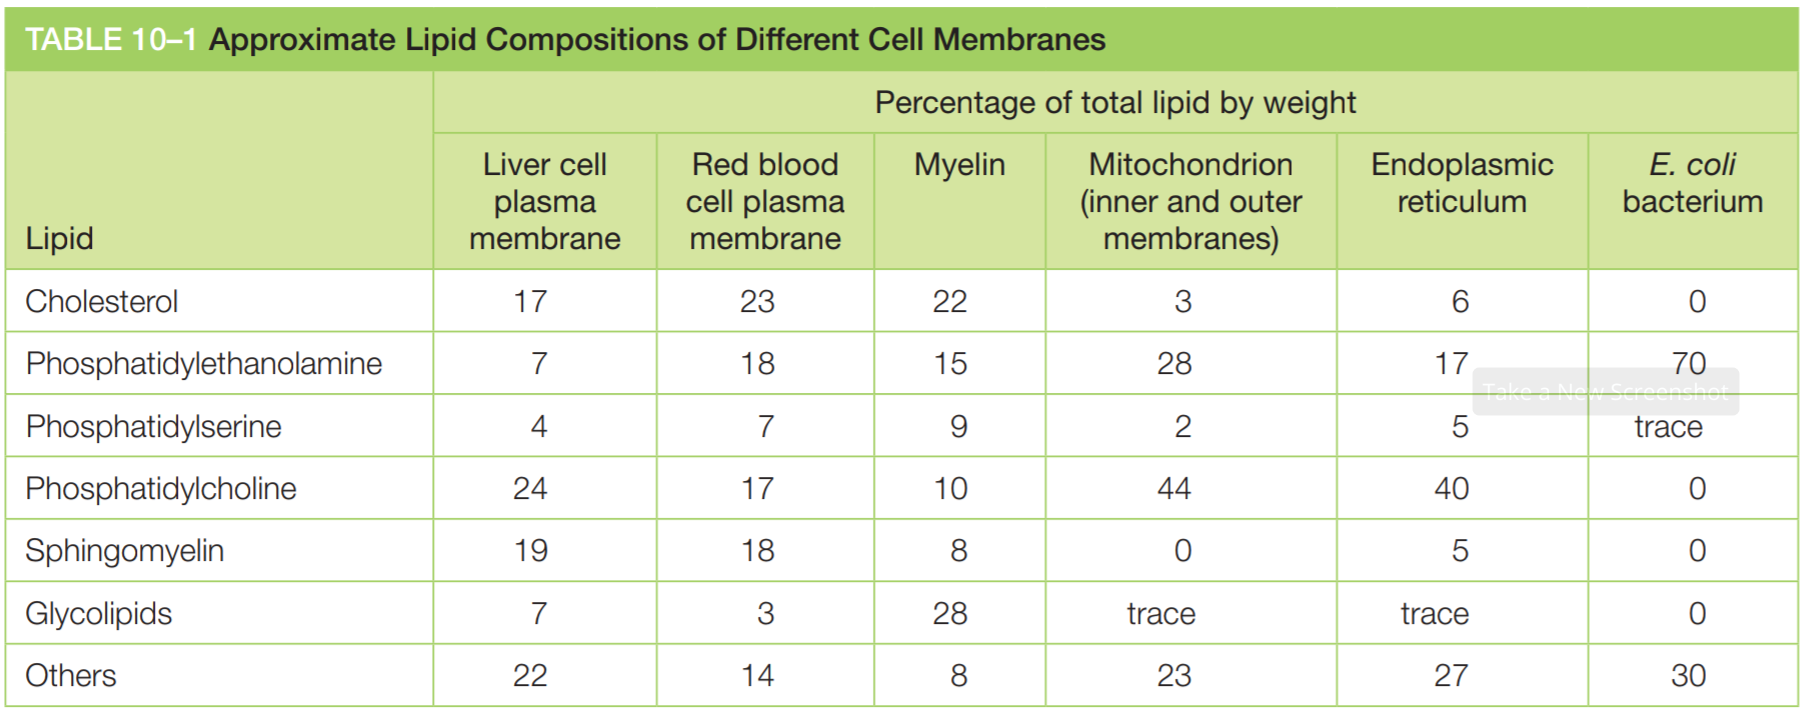
\includegraphics[width=\linewidth]{images/table_10_1.png}
    \end{itemize}

    \hypertarget{10.3}{\subsection*{Despite Their Fluidity, Lipid Bilayers Can Form Domains of Different Compositions}}
    \begin{itemize}
        \item \textbf{Lipid raft}: specialized domains, or regions, that are enriched with particular lipids and cholesterol that allow for specialized associations with different cellular proteins. 
        \item Lipid rafts are dynamic structures, often coming together or splitting apart.\
        \item Lipid rafts influence membrane fluidity and membrane protein trafficking,
        \item Although more common in the cell membrane, lipid rafts have also been reported in other parts of the cell, such as the Golgi apparatus and lysosomes.
    \end{itemize}

    \hypertarget{10.4}{\subsection*{Lipid Droplets Are Surrounded by a Phospholipid Monolayer}}
    \begin{itemize}
        \item \textbf{Lipid droplets}: lipid-rich cellular organelles that regulate the storage and hydrolysis of neutral lipids and are found largely in the adipose (fat) tissue. 
        \item Lipid droplets also serve as a reservoir for cholesterol and acyl-glycerols for membrane formation and maintenance.
        \item Generally, lipid droplets form rapidly in high concentration of fatty acids and generally form from discrete regions of the endoplasmic reticulum membrane where many enzymes of lipid metabolism are concentrated.
    \end{itemize}

    \hypertarget{10.5}{\subsection*{The Asymmetry of the Lipid Bilayer Is Functionally Important}}
    \begin{itemize}
        \item The lipid compositions of the two monolayers of the lipid bilayer in many membranes are strikingly different.
        \item Lipid asymmetry is functionally important, especially in converting extracellular signals into intracellular ones, as many cytosolic proteins bind to specific lipid head groups found in the cytosolic monolayer of the lipid bilayer. 
        \item Animals exploit the phospholipid asymmetry of their plasma membranes to
        distinguish between live and dead cells. 
    \end{itemize}
    
    \hypertarget{10.6}{\subsection*{Glycolipids Are Found on the Surface of All Eukaryotic Plasma Membranes}}
    \begin{itemize}
        \item \textbf{Glycolipids}: lipids with a carbohydrate attached by a glycosidic (covalent) bond.
        \item Glycolipids maintain the stability of the cell membrane and to facilitate cellular recognition, and are found on the surface of probably all eukaryotic cell membranes, where they extend from the phospholipid bilayer into the extracellular environment. 
        \item Glycolipids generally constitute about 5\% of the lipid molecules in the outer monolayer. 
        \item \textbf{Gangliosides}: a glycolipid that contain oligosaccharides (a polymer contain typically three to ten monosaccharides) with one or more sialic acid (an acidic sugar with a nine-carbon backbone), which produce a net negative charge.
        \item  Gangliosides are found predominantly in the nervous system where they constitute 6\% of all phospholipids.
    \end{itemize}

    \begin{probbox}{The Lipid Bilayer: Summary}
        Biological membranes consist of a continuous double layer of lipid molecules in which membrane proteins are embedded. This lipid bilayer is fluid, with individual lipid molecules able to diffuse rapidly within their own monolayer. The membrane lipid molecules are amphiphilic. When placed in water, they assemble spontaneously into bilayers, which form sealed compartments. Although cell membranes can contain hundreds of different lipid species, the plasma membrane in animal cells contains three major classes—phospholipids, cholesterol, and glycolipids. Because of their different backbone structure, phospholipids fall into two subclasses—phosphoglycerides and sphingolipids. The lipid compositions of the inner and outer monolayers are different, reflecting the different functions of the two faces of a cell membrane. Different mixtures of lipids are found in the membranes of cells of different types, as well as in the various membranes of a single eukaryotic cell. Inositol phospholipids are a minor class of phospholipids, which in the cytosolic leaflet of the plasma membrane lipid bilayer play an important part in cell signaling: in response to extracellular signals, specific lipid kinases phosphorylate the head groups of these lipids to form docking sites for cytosolic signaling proteins, whereas specific phospholipases cleave certain inositol phospholipids to generate small intracellular signaling molecules.
    \end{probbox}
}\end{secbox}
%  ^^^^^^^^^^^^^^^^^^^^^^^^^^^^^^^^^   Section 10.1   ^^^^^^^^^^^^^^^^^^^^^^^^^^^^^^^^  %  
%%%%%%%%%%%%%%%%%%%%%%%%%%%%%%%%%%%%%%%%%%%%%%%%%%%%%%%%%%%%%%%%%%%%%%%%%%%%%%%%%%%%%%%%%%
%  vvvvvvvvvvvvvvvvvvvvvvvvvvvvvvvvvv  Section 10.2   vvvvvvvvvvvvvvvvvvvvvvvvvvvvvvvv  % 
\hypertarget{10.2a}{}
\begin{secbox}{\hyperlink{10}{Membrane Proteins}}{
    \hypertarget{10.7}{\subsection*{Membrane Proteins Can Be Associated with the Lipid Bilayer in Various Ways}}
    \begin{itemize}
        \item \textbf{Membrane proteins}: amphiphilic proteins that are part of, or interact with, biological membranes. 
        \item Membrane proteins fall into several broad categories depending on their location, and classified generally as either integral or peripheral.
        \item Integral membrane proteins are a permanent part of a cell membrane and can either penetrate the membrane (transmembrane) or associate with just a single side of a membrane (integral monotopic).
        \item \textbf{Transmembrane protein}: a type of integral membrane protein that spans the entirety of the cell membrane.
        \item Transmembrane proteins are usually highly hydrophobic and aggregate and precipitate in water.
        \item Depending on the number of transmembrane segments, transmembrane proteins can be classified as single-span (or bitopic) or multi-span (polytopic).
        \item \textbf{Glycosylphosphatidylinositol (GPI) anchor}: a phosphoglyceride that can be attached to the C-terminus of a protein.
        \item The two fatty acids within the hydrophobic phosphatidyl-inositol group GPI anchor the protein to the cell membrane; leaving the protein bound to the noncytosolic surface of the ER membrane solely by this anchor.
        \item \textbf{Membrane-associated proteins}: proteins that do not extend into the hydrophobic interior of the lipid bilayer at all; they are instead bound to either face of the membrane by noncovalent interactions with other membrane proteins.\par
        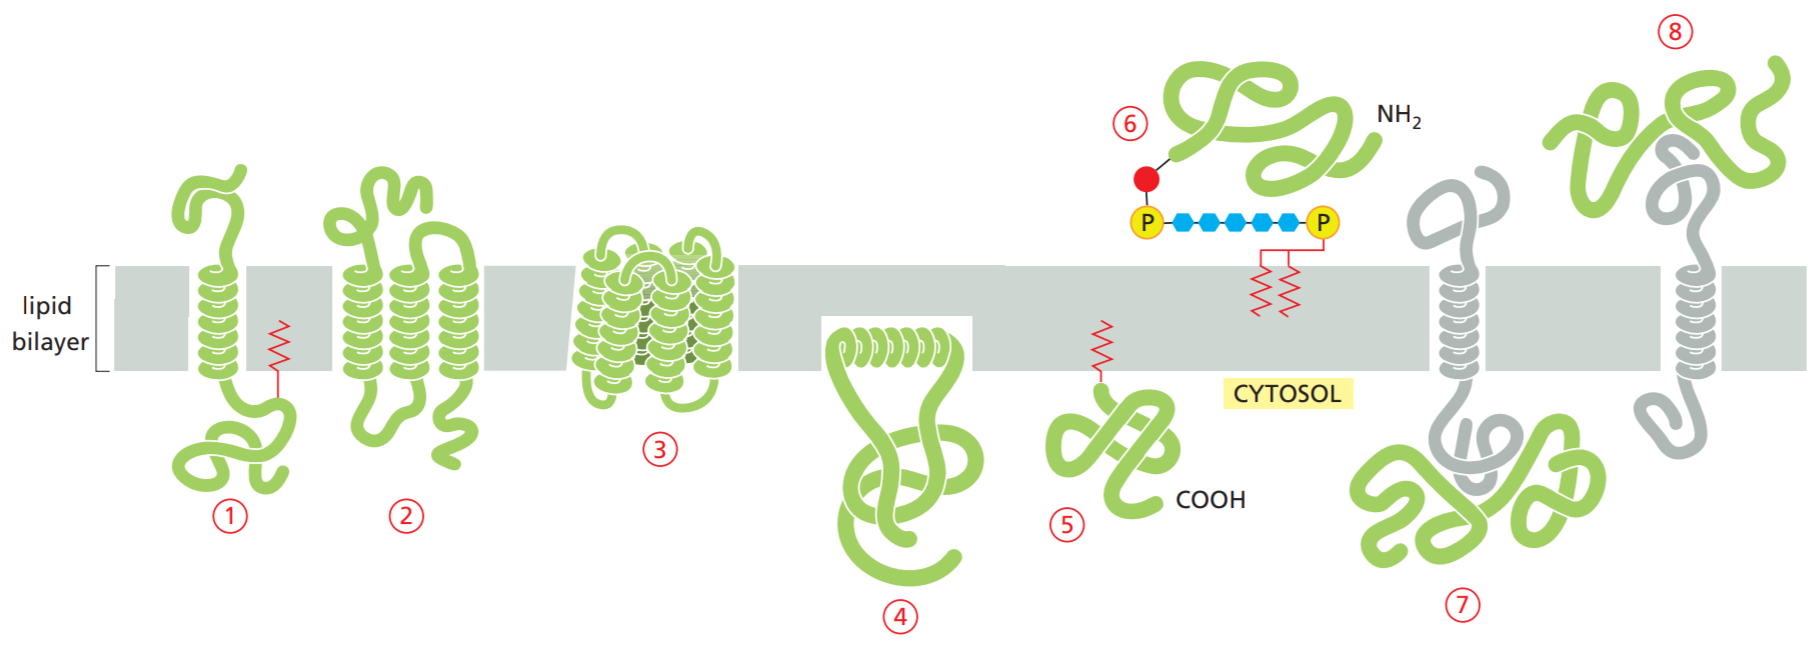
\includegraphics[width=\linewidth]{images/figure_10_17.png}
        \item \textcolor{red}{(1)} a single \(\alpha\) helix
        \item \textcolor{red}{(2)} as multiple \(\alpha\) helices
        \item \textcolor{red}{(3)} as a rolled-up \(\beta\) sheet (a \(\beta\) barrel). 
        \item \textcolor{red}{(4)} Some of these are anchored to the cytosolic surface by an amphiphilic \(\alpha\) helix that partitions into the cytosolic monolayer of the lipid bilayer through the hydrophobic face of the helix. 
        \item \textcolor{red}{(5)} Others are attached to the bilayer solely by a covalently bound lipid chain—either a fatty acid chain or a phenyl group in the cytosolic monolayer.
        \item \textcolor{red}{(6)} via an oligosaccharide linker, to phosphatidylinositol in the noncytosolic monolayer—called a GPI anchor. 
        \item \textcolor{red}{(7, 8)} membrane-associated proteins are attached to the membrane only by noncovalent interactions with other membrane proteins.
    \end{itemize}
    
    \hypertarget{10.8}{\subsection*{Lipid Anchors Control the Membrane Localization of Some Signaling Proteins}}
    \begin{itemize}
        \item \textit{Prenyl groups}: usually to facilitate attachment to cell membranes, similar to lipid anchors like the GPI anchor. Also can be done by a fatty acid chain.
        \item Prenyl groups have been shown to be important for protein–protein binding through specialized prenyl-binding domains.
    \end{itemize}
    
    \hypertarget{10.9}{\subsection*{In Most Transmembrane Proteins, the Polypeptide Chain Crosses the Lipid Bilayer in an \(\bm{\alpha}\)-Helical Conformation}}
    \begin{itemize}
        \item \textbf{Single pass transmembrane proteins} \textcolor{red}{(1)}: also known as bitopic proteins, which are transmembrane proteins that span the lipid bilayer only one time. 
        \item Bitopic proteins may constitute up to 50\% of all transmembrane proteins, depending on the organism, and contribute significantly to the network of interactions between different proteins in cells, including interactions via transmembrane helices.
        \item \textbf{Multi-pass transmembrane proteins} \textcolor{red}{(2)}: also known as polytopic proteins, where the polypeptide chain crosses membrane multiple times. 
    \end{itemize}

    \hypertarget{10.10}{\subsection*{Some \bfg{\beta} Barrels Form Large Channels}}
    \begin{itemize}
        \item The number of \(\beta\)-strands in a \(\beta\)-barrel varies widely, from as few as 8 strands to as many as 22
        \item \(\beta\)-barrel proteins are abundant in the outer membranes of bacteria, mitochondria, and chloroplasts.
        \item \textbf{Lumen}: a membrane-defined space that is found inside several organelles, cellular components, or structures: thylakoid, endoplasmic reticulum, Golgi apparatus, lysosome, mitochondrion, or microtubule
        \item Loops of the polypeptide chain often protrude into the lumen of the channel, narrowing it so that only certain solutes can pass.
        \item Not all \(\beta\)-barrel proteins are transport proteins. Some form smaller barrels that are completely filled by amino acid side chains that project into the center of the barrel. These proteins function as receptors or enzymes.
    \end{itemize}

    \hypertarget{10.11}{\subsection*{Many Membrane Proteins Are Glycosylated}}
    \begin{itemize}
        \item \textbf{Carbohydrate layer}: also known as, glycocalyx or the pericellular matrix, is a glycoprotein and glycolipid covering that surrounds the cell membranes of some bacteria, epithelia, and other cells.
        \begin{center}
            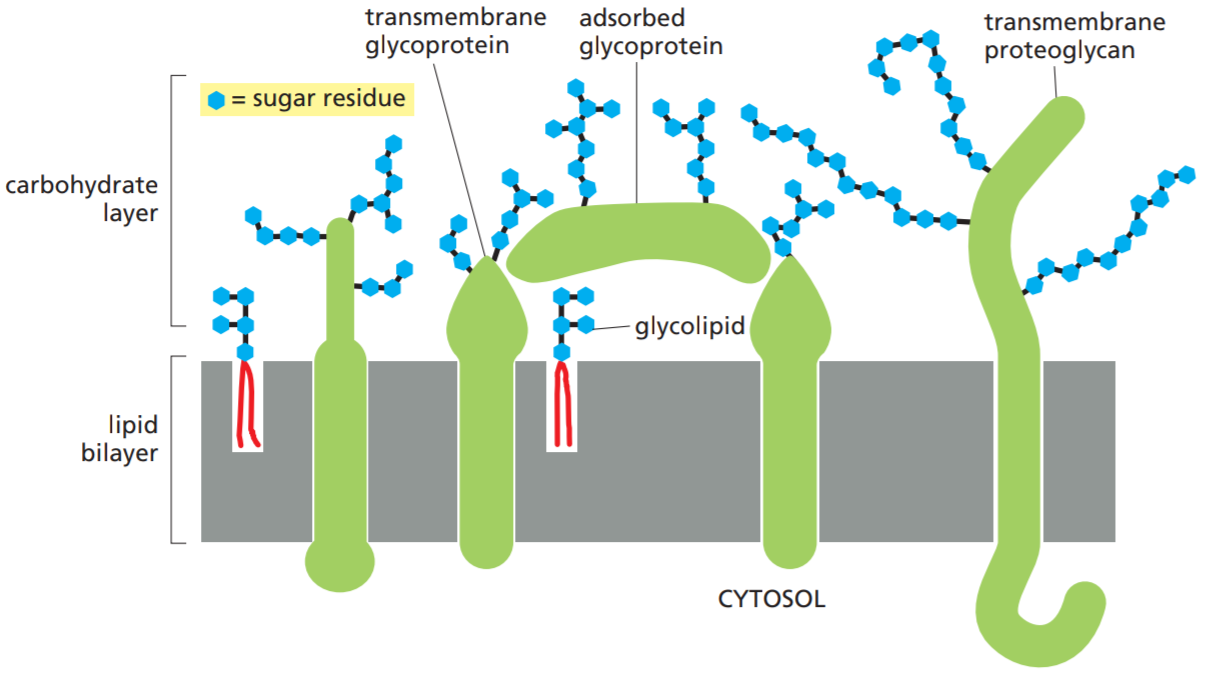
\includegraphics[scale=0.45]{images/figure_10_25.png}
        \end{center}
        \vspace{-20pt}
        \item The carbohydrate layer is made up of the oligosaccharide side chains of membrane glycolipids and membrane glycoproteins and the polysaccharide chains on membrane proteoglycans. In addition, adsorbed glycoproteins, and adsorbed proteoglycans (not shown), contribute to the carbohydrate layer in many cells.
        \item \textbf{Lectins}: carbohydrate-binding proteins that are highly specific for sugar groups of other molecules.\par 
        \item Lectins have a role in recognition on the cellular and molecular level and play numerous roles in biological recognition phenomena involving cells, carbohydrates, and proteins. 
    \end{itemize}

    \hypertarget{10.12}{\subsection*{Membrane Proteins Can Be Solubilized and Purified in Detergents}}
    \begin{itemize}
        \item \textbf{Detergents}: are small amphiphilic molecules of variable structure that disrupt hydrophobic associations and destroy the lipid bilayer, which can solubilize membrane proteins.
        \item At low concentration, detergents are monomeric in solution, but when their concentration is increased above a threshold, called the critical micelle concentration (CMC), they aggregate to form micelles.
        \item When mixed with membranes, the hydrophobic ends of detergents bind to the hydrophobic regions of the membrane proteins, where they displace lipid molecules with a collar of detergent molecules.
    \end{itemize}

    \hypertarget{10.13}{\subsection*{Bacteriorhodopsin Is a Light-driven Proton H\bfg{^+} Pump That Traverses the Lipid Bilayer as Seven \bfg{\alpha} Helices}}
    \begin{itemize}
        \item \textbf{Bacteriorhodopsin}: a protein used by Archaea, most notably by halobacteria, a class of the Euryarchaeota.
        \item Bacteriorhodopsin acts as a proton pump; that is, it captures light energy and uses it to move protons across the membrane out of the cell.
    \end{itemize}

    \hypertarget{10.14}{\subsection*{The Cortical Cytoskeleton Gives Membranes Mechanical Strength and Restricts Membrane Protein Diffusion}}
    \begin{itemize}
        \item \textbf{Spectrin}: a long, thin, flexible rod about 100 nm in length and is a cytoskeletal protein that lines the intracellular side of the plasma membrane in eukaryotic cells.  
        \item \textbf{Cortex}: also known as the actin cortex or actomyosin cortex, is a specialized layer of cytoplasmic proteins on the inner face of the cell membrane.
        \item The protein constituents of the cortex undergo rapid turnover, making the cortex both mechanically rigid and highly plastic, two properties essential to its function.
    \end{itemize}

    \hypertarget{10.15}{\subsection*{Membrane-bending Proteins Deform Bilayers}}
    \begin{itemize}
        \item In many cases, membrane shape is influenced by dynamic pushing and pulling forces exerted by cytoskeletal or extracellular structures.
        \item \textbf{Membrane bending proteins}: Proteins that control membrane curvature and play a crucial part in producing deformations needed to create cell structures.
        \item Currently there are 4 (the book lists 3) proposed mechanisms to explain protein-mediated membrane bending:
            \begin{itemize}[label=$\circ$]
                \item Lipid clustering: Bacterial toxins that favor binding, and thus clustering of certain lipid molecules, give rise to membrane curvature when factoring particular lipids involved.
                \item Protein forms rigid scaffold: proteins that deform the membrane or stabilize an already bent membrane.
                \item Insertion of amphipathic domains: Some insert hydrophobic protein domains or attached lipid anchors into one of the leaflets of a lipid bilayer. Increasing the area of only one leaflet causes the membrane to bend.
                \item Protein crowding (not in book): When a high enough local concentration of protein is present on membrane surface, repulsion between protein molecules on the membrane surface can induce membrane curvature. A recent study even shows that protein crowding can cause membrane bending and leads to membrane fission.
            \end{itemize}
        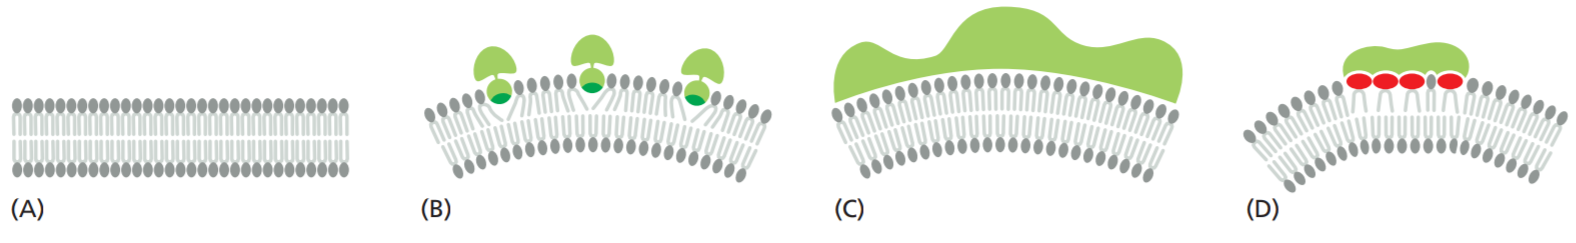
\includegraphics[width=\linewidth]{images/figure_10_40.png}
        \item (A) Bilayer without protein bound. 
        \item (B) A hydrophobic region of the protein can insert as a wedge into one monolayer to pry lipid head groups apart. Such regions can either be amphiphilic helices as shown or hydrophobic hairpins. 
        \item (C) The curved surface of the protein can bind to lipid head groups and deform the membrane or stabilize its curvature. 
        \item (D) A protein can bind to and cluster lipids that have large head groups and thereby bend the membrane. 
    \end{itemize}

    \begin{probbox}{Membrane Proteins: Summary}
        Whereas the lipid bilayer determines the basic structure of biological membranes, proteins are responsible for most membrane functions, serving as specific receptors, enzymes, transporters, and so on. Transmembrane proteins extend across the lipid bilayer. Some of these membrane proteins are single-pass proteins, in which the polypeptide chain crosses the bilayer as a single \(\alpha\)-helix. Others are multipass proteins, in which the polypeptide chain crosses the bilayer multiple times---either as a series of \(\alpha\)-helices or as a \(\beta\)-sheet rolled up into the shape of a barrel. All proteins responsible for the transport of ions and other small water-soluble molecules through the membrane are multipass proteins. Some membrane proteins do not span the bilayer but instead are attached to either side of the membrane: some are attached to the cytosolic side by an amphipathic a helix on the protein surface or by the covalent attachment of one or more lipid chains, others are attached to the noncytosolic side by a GPI anchor. Some membrane-associated proteins are bound by noncovalent interactions with transmembrane proteins. In the plasma membrane of all eukaryotic cells, most of the proteins exposed on the cell surface and some of the lipid molecules in the outer lipid monolayer have oligosaccharide chains covalently attached to them. Like the lipid molecules in the bilayer, many membrane proteins are able to diffuse rapidly in the plane of the membrane. However, cells have ways of immobilizing specific membrane proteins, as well as ways of confining both membrane protein and lipid molecules to particular domains in a continuous lipid bilayer. The dynamic association of membrane-bending proteins confers on membranes their characteristic three-dimensional shapes.
    \end{probbox}
}\end{secbox}
%\endgroup
%  ^^^^^^^^^^^^^^^^^^^^^^^^^^^^^^^^^    Chapter 11    ^^^^^^^^^^^^^^^^^^^^^^^^^^^^^^^^^  %  
%%%%%%%%%%%%%%%%%%%%%%%%%%%%%%%%%%%%%%%%%%%%%%%%%%%%%%%%%%%%%%%%%%%%%%%%%%%%%%%%%%%%%%%%%%

%%%%%%%%%%%%%%%%%%%%%%%%%%%%%%%%%%%%%%%%%%%%%%%%%%%%%%%%%%%%%%%%%%%%%%%%%%%%%%%%%%%%%%%%%%
%  vvvvvvvvvvvvvvvvvvvvvvvvvvvvvvvvv    Chapter 11    vvvvvvvvvvvvvvvvvvvvvvvvvvvvvvvvv  %
%\begingroup

\clearpage
\renewcommand{\thetitle}{\hypertarget{11}{Transport Across Membranes}}
\rfoot{\hyperlink{11}{11 --- \thepage}}
\hypertarget{11}{}

\begin{chapbox}{\hyperlink{home}{Chapter 11: Transport Across Membranes}}
    \begin{enumerate}
        \item \hyperlink{11.1}{Principles of Membrane Transport}
            \begin{itemize}
                \item \hyperlink{11.1.1}{Transporters and Channels}
                \item \hyperlink{11.1.2}{Active Transport Mediation}
                \item \hyperlink{11.1.r}{Summary}
            \end{itemize}
        \item \hyperlink{11.2}{Transporters and Active Membrane Transport}
            \begin{itemize}
                \item \hyperlink{11.2.1}{Ion-concentration Gradients}
                \item \hyperlink{11.2.2}{Transcellular Transport of Solutes}
                \item \hyperlink{11.2.3}{ATP-Driven Pumps}
                \item \hyperlink{11.2.4}{P-type ATPase, \ch{Ca^2+}, and the Sarcoplasmic Reticulum in Muscle Cells}
                \item \hyperlink{11.2.5}{Gradients Across the PLasma Membrane}
                \item \hyperlink{11.2.6}{ABC Transporters}
                \item \hyperlink{11.2.r}{Summary}
            \end{itemize}
        \item \hyperlink{11.3}{Channels and the Electrical Properties of Membranes}
            \begin{itemize}
                \item \hyperlink{11.3.1}{Aquaporins Are Permeable to Water But Impermeable to Ions}
                \item \hyperlink{11.3.2}{Ion Channels Are Ion-Selective and Fluctuate Between Open and Closed States}
                \item \hyperlink{11.3.3}{Membrane Potential in Animal Cells}
                \item \hyperlink{11.3.4}{Three-Dimensional Structure of a Bacterial \ch{K^+} Channel}
                \item \hyperlink{11.3.5}{Mechanosenstive Channels}
                \item \hyperlink{11.3.6}{Neuron Function}
                \item \hyperlink{11.3.7}{Voltage-Gated Cation Channels}
                \item \hyperlink{11.3.8}{Channelrhodopsins}
                \item \hyperlink{11.3.9}{Myelination}
                \item \hyperlink{11.3.10}{Patch-Clamp Recording}
                \item \hyperlink{11.3.11}{Voltage-Gated Cation Channels}
                \item \hyperlink{11.3.12}{Transmitter-Gated Ion Channels}
                \item \hyperlink{11.3.13}{Chemical Synapses Can Be Excitatory or Inhibitory}
                \item \hyperlink{11.3.14}{Excitatory Transmitter-Gated Cation Channels}
                \item \hyperlink{11.3.15}{More on Neurons}
                \item \hyperlink{11.3.16}{Neuromuscular Transmission}
                \item \hyperlink{11.3.17}{Neuronal Computation}
                \item \hyperlink{11.3.18}{Long-Term Potentiation (LTP) in the Mammalian Hippocampus}
                \item \hyperlink{11.3.r}{Summary}
            \end{itemize}
    \end{enumerate}
\end{chapbox}

\hypertarget{11.1}{}
\begin{secbox}{\hyperlink{11}{Principles of Membrane Transport}}{
    \begin{itemize}
        \item Up to 15-30\% of the membrane proteins in all cells are transmembrane transport proteins. 
        \item Small nonpolar molecules, such as \ch{O2} and \ch{CO2} readily dissolve in lipid bilayers.
    \end{itemize}
    \begin{center}
        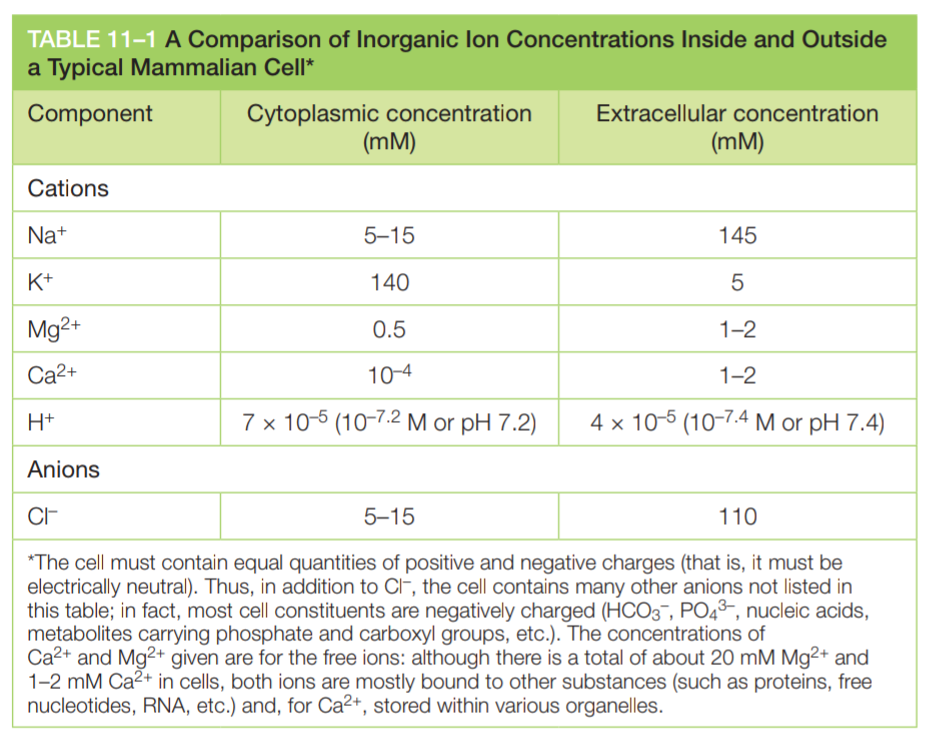
\includegraphics[scale=0.4]{images/tab11-1.png}
    \end{center}
    \vspace{-1cm} 
    \hypertarget{11.1.1}{\subsection*{Transporters and Channels}}
    \begin{itemize}
        \item \textbf{Membrane transport proteins (MTPs)}: proteins specialized in transporting solutes such as ions, sugar, amino acids, nucleotides, water, and more. 
        \item In the 1950s some bacteria with a single-gene mutation were able to break transport proteins, suggesting many transport proteins have high specificity.
        \item All membrane transporter proteins have been polytopic.
        \item There are two major classes of MTPs, transporters and channels.
        \item \textbf{Transporters}: also called carriers or permeases, are not open simultaneously to both the extracellular and intracellular environments. Either its inner gate is open, or outer gate is open.
        \item \textbf{Channels}: form continuous pores that open to both environments at the same time, allowing the molecules to diffuse without interruption.
    \end{itemize}

    \hypertarget{11.1.2}{\subsection*{Active Transport Mediation}}
    \begin{itemize}
        \item \textbf{Passive transport}: also known as facilitated diffusion, involves the use of an electrochemical gradient, and does not use energy produced in the cell.
        \item \textbf{Electrochemical gradient}: a gradient of electrochemical potential, usually for an ion that can move across a membrane. The gradient consists of two parts, the chemical gradient, or difference in solute concentration across a membrane, and the electrical gradient, or difference in charge across a membrane.
        \item \textbf{Active transport}: also called primary active transport, is the movement of a substance across a membrane against its concentration gradient that uses metabolic energy, such as ion gradient or ATP hydrolysis.
        \item \textbf{Secondary active transport}: utilizes passive transport, but first uses ATP-pumps to create electrochemical gradients, thus indirectly facilitating transport. 
    \end{itemize} 
    \vspace{6pt}
    \hypertarget{11.1.r}{}
    \begin{probbox}{Principles of Membrane Transporter: Summary}\end{probbox}
    \vspace{18pt}
        Lipid bilayers are virtually impermeable to most polar molecules. To transport small water-soluble molecules into or out of cells or intracellular membrane-enclosed compartments, cell membranes contain various membrane transport proteins, each of which is responsible for transferring a particular solute or class of solutes across the membrane. There are two classes of membrane transport proteins—transporters and channels. Both form protein pathways across the lipid bilayer. Whereas transmembrane movement mediated by transporters can be either active or passive, solute flow through channel proteins is always passive. Both active and passive ion transport is influenced by the ion’s concentration gradient and the membrane potential--that is, its electrochemical gradient.
}\end{secbox}

\hypertarget{11.2}{}
\begin{secbox}{\hyperlink{11}{Transporters and Active Membrane Transport}}{
    \begin{itemize}
        \item Cells carry out active transport to pump a solute against its electrochemical gradient in three main ways:
            \begin{itemize}
                \item \textit{Coupled transporters}: coupling of one solute to that goes uphill against with one that goes downhill.
                \item \textit{ATP-driven pumps}: couple uphill transport to the hydrolysis of ATP.
                \item \textit{Light- or redox-driven pumps}: known in bacteria, archaea, mitochondria, and chloroplasts, use light, as with bacteriorhodopsin, or from a redox reaction (such as cytochrome c oxidase).
            \end{itemize}
    \end{itemize}
    \hypertarget{11.2.1}{\subsection*{Ion-concentration Gradients}}
    \begin{itemize}
        \item \textbf{Uniporters}: passive mediation of the movement of a single solute and regulated by voltage, stress, or through ligands. 
        \item \textbf{Symporters}: also known as coupled transporters, involved the simultaneous transfer of a second solute in the same direction. 
        \item \textbf{Antiporters}: also called exchangers, is similar to symporters, but instead transport solutes in the opposite direction.
        \item An electrochemical \ch{H^+} gradient across the bacterial plasma membrane, for example, drives the inward active transport of many sugars and amino acids. 
    \end{itemize}

    \hypertarget{11.2.2}{\subsection*{Transcellular Transport of Solutes}}
    \begin{itemize}
        \item \textbf{Transcellular transport}: involves the transportation of solutes by a cell through a cell.
    \end{itemize}

    \hypertarget{11.2.3}{\subsection*{ATP-Driven Pumps}}
    \begin{itemize}
        \item ATP-driven pumps are often called transport ATPases because they hydrolyze ATP to ADP and phosphate and use the energy released to pump ions or other solutes across a membrane.
        \item There are three principal classes:
        \begin{itemize}
            \item \textbf{P-type pumps}: include many of the ion pumps responsible for setting up and maintaining gradients. Known as P-type because they phosphorylate themselves during the pumping cycle.
            \item \textbf{ABC transporters}: primarily pump small molecules across cell membranes.
            \item \textbf{V-type pumps}: turbine-like machines, constructed form multiple different subunits, used to pump protons into organelles. F-type is the inverse of V-type.
        \end{itemize}
        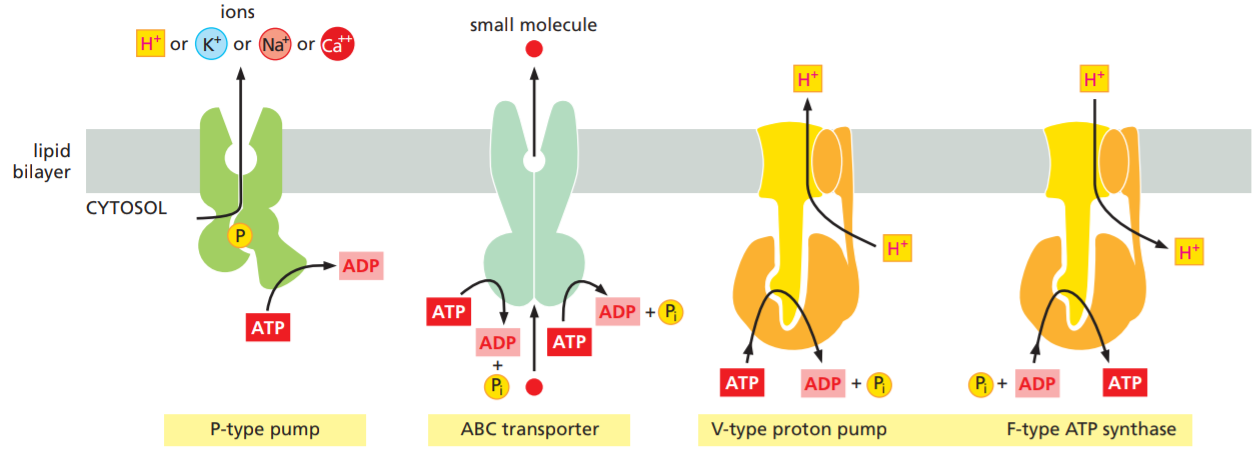
\includegraphics[width=\linewidth]{images/fig11-12.png}
    \end{itemize}
    \hypertarget{11.2.4}{\subsection*{P-type ATPase, \ch{Ca^2+}, and the Sarcoplasmic Reticulum in Muscle Cells}}
    \begin{itemize}
        \item \textit{Sarcoplasmic reticulum (SR)}: a specialized type of endoplasmic reticulum that forms a network of tubular sacs in the muscle cell cytoplasm, and it serves as an intracellular store of \ch{Ca^2+}.
        \item \textbf{\ch{Ca^2+} ATPase}: a well understood pump in the SR membrane of skeletal muscle cells.
    \end{itemize}

    \hypertarget{11.2.5}{\subsection*{Gradients Across the PLasma Membrane}}
    \begin{itemize}
        \item The concentration of \ch{K^+} is typically 10–30 times higher inside cells than outside, whereas the reverse is true of \ch{Na^+}.
        \item \textbf{\ch{Na^+ -K^+} ATPase}, or \ch{Na^+ -K^+} pump, is found in the plasma membrane of virtually all animal cells and maintains these concentration differences.
        \item  The \ch{Na^+ -K^+} pump uses 3 positively charges ions for every 2 it pumps in. This makes it \textit{electrogenic}, meaning it changes or creates a electrical potential of a cell. 
        \item This electrogenic effect seldomly contributes more than 10\% to the membrane potential.
    \end{itemize}
    
    \hypertarget{11.2.6}{\subsection*{ABC Transporters}}
    \begin{itemize}
        \item \textbf{ATP-Binding Cassettes}: two highly conserved ATPase domains on the cytosolic side of the membrane.
        \item ATP binding brings together the two ATPase domains, and ATP hydrolysis leads to their dissociation, which ABC transporters harvest and use to drive transport of solutes across the bilayer.
        \item ABC transporters are a superfamily and is one of the largest and possibly one of the oldest gene families.
        \item \textbf{Multidrug resistance (MDR) protein}: the first eukaryotic ABC transporters identified and have an ability to pump hydrophobic drugs out of the cytosol.
    \end{itemize}
    
    \begin{probbox}{Transporters and Active Membrane Transport: Summary}\end{probbox}
        Transporters bind specific solutes and transfer them across the lipid bilayer by undergoing conformational changes that alternately expose the solute-bindingsite on one side of the membrane and then on the other. Some transporters move a single solute “downhill,” whereas others can act as pumps to move a solute“uphill” against its electrochemical gradient, using energy provided by ATPhydrolysis, by a downhill flow of another solute (such as Na + or H+), or by light to drive the requisite series of conformational changes in an orderly manner. Transporters belong to a small number of protein families. Each family evolved from a common ancestral protein, and its members all operate by a similar mechanism. The family of P-type transport ATPases, which includes Ca2+ and Na +-K+ pumps, is an important example; each of these ATPases sequentially phosphorylates and dephosphorylates itself during the pumping cycle. The superfamily of ABC transporters is the largest family of membrane transport proteins and is especially important clinically. It includes proteins that are responsible for cystic fibrosis, for drug resistance in both cancer cells and malaria-causing parasites, and for pumping pathogen-derived peptides into the ER for cytotoxic lymphocytes to reorganize on the surface of infected cells.
}\end{secbox}

\hypertarget{11.3}{}
\begin{secbox}{\hyperlink{11}{Channels and the Electrical Properties of Membranes}}{
    \hypertarget{11.3.1}{\subsection*{Aquaporins Are Permeable to Water But Impermeable to Ions}}
    \begin{itemize}
        \item \textbf{Ion channels}: proteins concerned specifically with inorganic ion transport.
        \item Ion channels can pas up to 100 million ions through one open channel each second. 10$^5$ time greater than the fastest known transporter. 
        \item Channels cannot be coupled to an energy source, so their mediation is always passive.
        \item \textbf{Aquaporins}: permeable to water but impermeable to ions.
        \item Aquaporins contain two strategically placed asparagines, which bind to the oxygen atom of the central water molecule in the line of water molecules traversing the pore, imposing a bipolarity on the entire column of water molecules.
    \end{itemize}

    \hypertarget{11.3.2}{\subsection*{Ion Channels Are Ion-Selective and Fluctuate Between Open and Closed States}}
    \begin{itemize}
        \item \textit{Ion selectivity}: of one the main property that allows ion channels to permit particular inorganic ions. This is done by a \textit{selectivity filter} that is applied to ions as they pass through the narrowest part of the channel.
        \item \textit{Gated}: the other main property that ion channels utilize by allowing the channels to open and close. 
        \item There are several types of stimuli that are know to be control gating. These include: voltage-gated channels, mechanically gated channels, ligand-gated channels--transmitter-gated, ion-gated, or nucleotide-gated--and even protein phosphorylation and dephosphoylation. 
        \item More than 100 types of ion channels have been identified. 
        \item A single neuron typically contains 10 or more kinds of ion channels.
        \item \textbf{\ch{K^+} leak channels}: ion channels that are permeable to mainly \ch{K^+} and that can open even in an unstimulated cell. 
    \end{itemize}

    \hypertarget{11.3.3}{\subsection*{Membrane Potential in Animal Cells}}
    \begin{itemize}
        \item \textbf{Membrane potential} arises when there is a difference in the electrical charge on the two sides of a membrane, due to a slight excess of positive ions over negative ones on one side and a slight deficit on the other. 
        \item Membrane potential can be made from active electrogenic pumping and passive ion diffusion.
        \item Passive ion movements make the largest contribution to membrane potential in typical animal cells.
        \item Membrane potential equilibrium can be calculated from the steepness of the \ch{K^+} concentration gradient.
        \item \textbf{Resting membrane potential}: the equilibrium condition, in which there is no net flow of ions across the plasma membrane.
        \item \textbf{Nernst equation}: quantifies the equilibrium condition and makes it possible to calculate the theoretical resting membrane potential if the ratio between internal and external ion concentration is known.
        \item The resting potential of an animal cell varies between -20 mV and -120 mV.
        \item The more permeable the membrane for a given ion, the more strongly the membrane potential tends to be driven toward the equilibrium value for that ion. 
        \item Changes in membranes permeability to ions can cause significant changes in membrane potential. 
    \end{itemize}

    \hypertarget{11.3.4}{\subsection*{Three-Dimensional Structure of a Bacterial \ch{K^+} Channel}}
    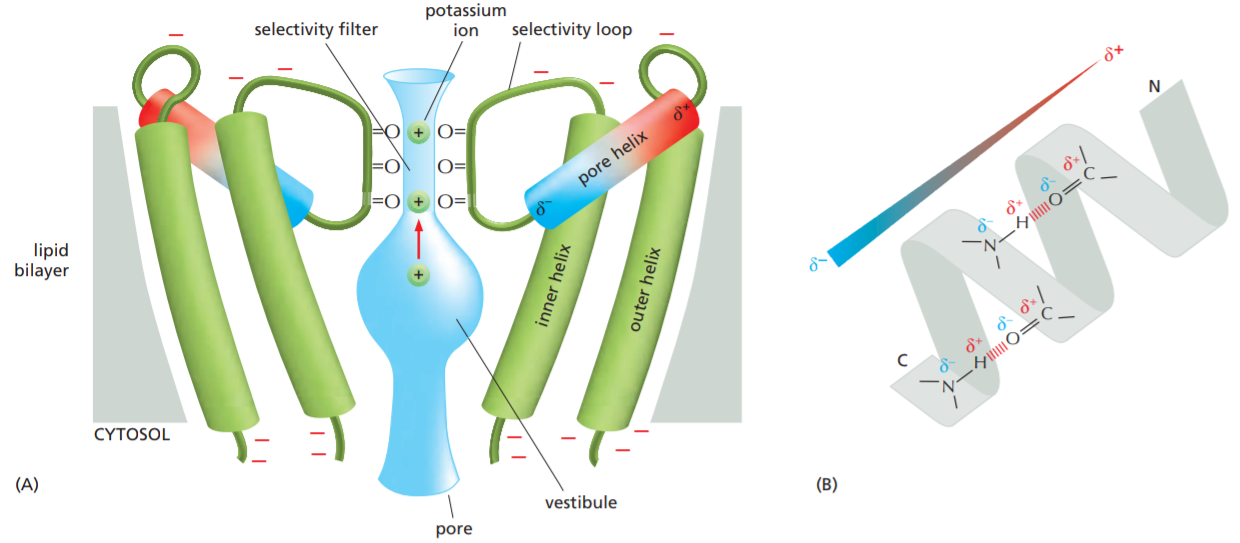
\includegraphics[width=\linewidth]{images/fig11-24.png}
    \begin{itemize}
        \item \textbf{Selectivity filter}: a polypeptide chain that connects two transmembrane helices to form a short \(\alpha\)-helix and a crucial loop that protrudes into the wide section of the cone. The selectivity loops from the four subunits to form a short, rigid, narrow pore, lined by carbonyl oxygen atoms.
    \end{itemize}

    \hypertarget{11.3.5}{\subsection*{Mechanosenstive Channels}}
    \begin{itemize}
        \item \textbf{Mechanosenstive channels}: are the sensors for a number of systems including the senses of touch, hearing and balance, as well as participating in cardiovascular regulation and osmotic homeostasis. 
    \end{itemize}

    \hypertarget{11.3.6}{\subsection*{Neuron Function}}
    \begin{itemize}
        \item \textbf{Neuron}: a cell tasked to receive, conduct, and transmit signals. 
        \item \textbf{Axon}: conducts signals away from he cell body.
        \item \textbf{Dendrites}: terminal branches of the axon used to connect to other cells. 
        \item \textbf{Action Potential}, or nerve impulse, can carry a message without attenuation at speeds of 100meters per second or more.
        \item Action potentials are the direct consequence of the properties of voltage-gated cation channels.
    \end{itemize}
    
    \hypertarget{11.3.7}{\subsection*{Voltage-Gated Cation Channels}}
    \begin{itemize}
        \item \textbf{Voltage-gated cation channels}: responsible for generating the action potentials
        \item \textbf{Depolarization}:  a shift in the membrane potential to a less negative value inside. 
        \item \textbf{Voltage-gated \ch{Na^+} channels}: opened by a stimulus in the nerve and skeletal muscle cells and the result of depolarization.
        \item \ch{Na^+} channels are an example of positive feedback that shifts the electrical potential of the local region from $\approx$ -70 mV to $\approx$ +50 mV.
        \item \ch{Na^+} channels automatically inactive. 
        \item \textbf{Voltage-gated \ch{K^+} channels}: channels that open in to restore membrane potential to its initial negative value.
        \item \textit{Refractory period}: the time required for \ch{Na^+} channels to recover from self inactivation and to support a new action potential. 
    \end{itemize}
    
    \hypertarget{11.3.8}{\subsection*{Channelrhodopsins}}
    \begin{itemize}
        \item \textbf{Channelrhodopsins}: photosensitive ion channels that open in response to light.
        \item channelrhodopsin can be expressed in virtually any cell type in vertebrates and invertebrates.
        \item \textbf{Optognetics}: a field in which neuroscientists attempt to analyze the neurons and circuits underlying even the most complex behaviors in experimental animals, including nonhuman primates.
    \end{itemize}
    
    \hypertarget{11.3.9}{\subsection*{Myelination}}
    \begin{itemize}
        \item \textbf{Myelin Sheath}: a sheath that surrounds axons of many vertebrate neurons that greatly increases the rate at which an axon can conduct an action potential.
        \item \textbf{Glial cells}: cells responsible for forming myelin. 
        \item \textbf{Schwann cells}: the glial cells that myelinate axons in peripheral nerves.
        \item \textbf{Oligodendrocytes}: glial cells that myelinate axons in the central nervous system.
        \item \textit{nodes of Ranvier}: regularly spaced nodes that interrupt the myeline sheath and where almost all \ch{Na^+} channels in the axon are concentrated.
        \item \textit{Saltatory conduction}: the process in which action potential propagate along myelinated axon by jumping from node to node. This allows for much faster and greater metabolic efficiency.
    \end{itemize}
    
    \hypertarget{11.3.10}{\subsection*{Patch-Clamp Recording}}
    \begin{itemize}
        \item \textbf{Patch-clamp recording}: a technique that makes it possible to record current flowing through individual channels.
    \end{itemize}

    \hypertarget{11.3.11}{\subsection*{Voltage-Gated Cation Channels}}
    \begin{itemize}
        \item \ch{Na^+} channels are not the only kind of voltage-gated cation channel that can generate an action potential.
        \item The action potentials in some muscle, egg, and endocrine cells, for example, depend on voltage-gated \ch{Ca^2+} channels rather than on \ch{Na^+} channels. 
        \item The particular combination of ion channels conducting \ch{Na^+}, \ch{K^+}, and \ch{Ca^2+} that are expressed in a neuron largely determines how the cell fires repetitive sequences of action potentials. Some nerve cells can repeat action potentials up to 300 times per second; other neurons fire short bursts of action potentials separated by periods of silence; while others rarely fire more than one action potential at a time.
    \end{itemize}
    
    \hypertarget{11.3.12}{\subsection*{Transmitter-Gated Ion Channels}}
    \begin{itemize}
        \item \textbf{Synapses}: specialized sites of contact that neuronal signals are transmitted from cell to cell.
        \item The \textit{presynaptic cell} is separated from the \textit{postsynaptic cell} by a narrow \textit{synaptic cleft}. 
        \item \textbf{Neurotransmitters}: small molecules released from membrane enclosed \textit{synaptic vesicles} by exocytosis. 
        \item Neurotransmitters diffuse rapidly across the synaptic cleft and provokes an electrical change in the postsynaptic cell by binding to and opening \textit{transmitter-gated ion channels}.
        \item \textbf{Transmitter-gated ion channels}: also known as ionotropic receptors, and are used for rapidly converting extracellular chemical signals into electrical signals at chemical synapses.
    \end{itemize}
    
    \hypertarget{11.3.13}{\subsection*{Chemical Synapses Can Be Excitatory or Inhibitory}}
    \begin{itemize}
        \item \textbf{Excitatory neurotransmitters}: open cation channels, causing an influx of \ch{NA^+}, and in  many cases \ch{Ca^2+}, that depolarizes the postsynaptic membrane toward the threshold potential for firing an action potential. 
        \item \textbf{Inhibitory neurotransmitters}: open either \ch{Cl^-} or \ch{K^+} channels, which suppresses firing by making it harder for excitatory neurotransmitters to depolarize the postsynaptic membrane. 
        \item \textbf{Metabotropic receptors}: regulate ion channels only indirectly through the action of small intracellular signal molecules. 
        \item All neurotransmitters receptors fall into two major classes--ionotropic or metabotropic.
        \item Ionotropic are ion channels and feature at fast chemical synapses that are immediate, simple, and brief.
        \item Metabotropic receptors are \textit{G-protein-coupled receptors} that bind to all other neurotransmitters and are usually slower, more complex, and longer lasting.
    \end{itemize}
    
    \hypertarget{11.3.14}{\subsection*{Excitatory Transmitter-Gated Cation Channels}}
    \begin{itemize}
        \item \textbf{Acetylcholine receptor}: a well studied example of transmitter-gated ion channel in the skeletal muscle cells. 
        \item \textbf{Neuromuscular junction}: the specialized chemical synapse between a motor neuron and a skeletal muscle cell.
    \end{itemize}

    \hypertarget{11.3.15}{\subsection*{More on Neurons}}
    \begin{itemize}
        \item For each class of transmitter-gated ion channel, there are alternative forms of each type of subunit, which may be encoded by distinct genes or else generated by alternative RNA splicing of a single gene product.
        \item  The subunits assemble in different combinations to form an extremely diverse set of distinct channel subtypes \item Subsets of such neurons performing different functions in the brain express different combinations of the genes for these subunits.
    \end{itemize}
    
    \hypertarget{11.3.16}{\subsection*{Neuromuscular Transmission}}
    \begin{itemize}
        \item Neuromuscular transmission requires the sequential activation of at least five different sets of ion channels.
        \begin{center}
            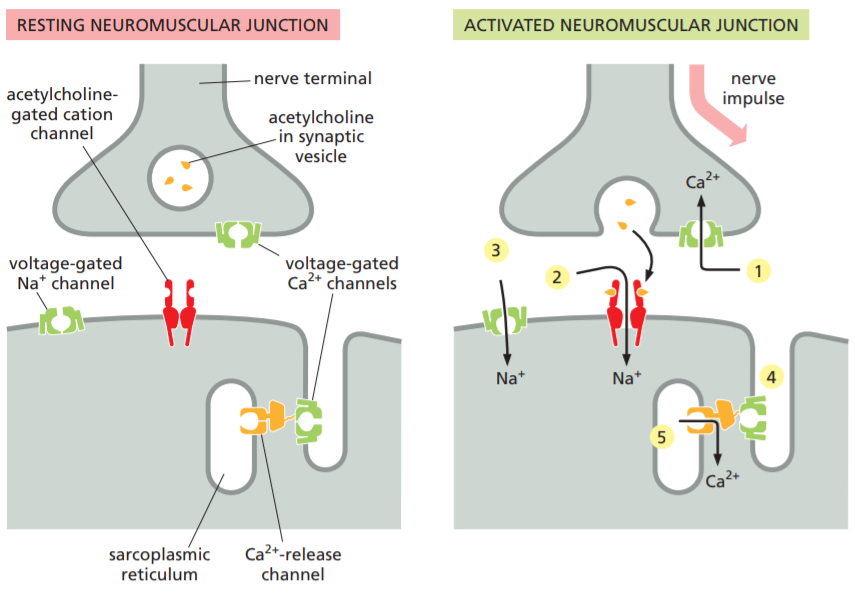
\includegraphics[scale=0.5]{images/fig11-39.png}
        \end{center}
    \end{itemize}
    \vspace{-1cm}

    \hypertarget{11.3.17}{\subsection*{Neuronal Computation}}
    \begin{itemize}
        \item \textbf{Initial segment}: a specialized region of the axonal membrane where encoding takes place and is located at the junction of the axon and the cell body.
        \item \textbf{Delayed \ch{K^+} channels}: voltage-gated channels that repolarizes the membrane after each action potential to prepare the cell to fire again.
        \item \textbf{Rapidly inactivating \ch{K^+} channels}: also voltage-gated, but their specific voltage sensitivity and kinetics of inactivation are such that they act to reduce the rate of firing at levels of stimulation that are only just above the threshold required for firing.
        \item The result is a firing rate that is proportional to the strength of the depolarizing stimulus over a very broad range.  
        \item \textbf{Adaptation}: a response of the cell to an unchanging, prolonged stimulation. 
        \item \textbf{\ch{Ca ^2+}-activated \ch{K^+} channel}: opened in response to a raised concentration of \ch{Ca^2+} at the channel's cytoplasmic face and makes the membrane harder to depolarize.
        \item \textbf{Synaptic plasticity}: a ability of individual synapses to strengthen or weaken depending on their use. 
    \end{itemize}
    
    \hypertarget{11.3.18}{\subsection*{Long-Term Potentiation (LTP) in the Mammalian Hippocampus}}
    \begin{itemize}
        \item \textbf{Long-term potentiation (LTP)}: caused by a short burst of repetitive firing, which causes subsequent single action potentials in the presynaptic cells evoke a greatly enhanced response in the postsynaptic cells.
        \item \textbf{AMPA receptors}: glutamate-gated ion channels responsible for the excitatory PSPs.
        \item \textbf{NMDA receptors}: a separate subclass of glutamate-gated ion channels that are selectively activated by the artificial glutamate analog N-methyl-D-aspartate. 
        \item NMDA are normally only be activated when AMPA receptors are activated as well and the membrane is strongly depolarized. 
        \item NMDA receptors mediate LTP.
        \item \textbf{Long-term depression (LTD)}: a long-term effect of reducing the number of AMPA receptors in the post-synaptic membrane.
    \end{itemize}
    
    \hypertarget{11.3.r}{}
    \begin{probbox}{Channels and the Electrical Properties of Membranes: Summary}\end{probbox}
        Ion channels form aqueous pores across the lipid bilayer and allow inorganic ions of appropriate size and charge to cross the membrane down their electrochemical gradients at rates about 1000 times greater than those achieved by any known transporter. The channels are “gated” and usually open transiently in response to a specific perturbation in the membrane, such as a change in membrane potential (voltage-gated channels), or the binding of a neurotransmitter to the channel (transmitter-gated channels).\par
        \vspace{12pt}
        \ch{K+}-selective leak channels have an important role in determining the resting membrane potential across the plasma membrane in most animal cells.  Voltage-gated cation channels are responsible for the amplification and propagation of action potentials in electrically excitable cells, such as neurons and skeletal muscle cells. Transmitter-gated ion channels convert chemical signals to electrical signals at chemical synapses. Excitatory neurotransmitters, such as acetylcholine and glutamate, open transmitter-gated cation channels and thereby depolarize the postsynaptic membrane toward the threshold level for firing an action potential. Inhibitory neurotransmitters, such as GABA and glycine, open transmitter-gated \ch{Cl^-} or \ch{K^+} channels and thereby suppress firing by keeping the postsynaptic membrane polarized. A subclass of glutamate-gated ion channels, called NMDA-receptor channels, is highly permeable to \ch{Ca^2+}, which can trigger the long-term changes in synapse efficacy (synaptic plasticity) such as LTP and LTD that are thought to be involved in some forms of learning and memory.\par 
        \vspace{12pt}
        Ion channels work together in complex ways to control the behavior of electrically excitable cells. A typical neuron, for example, receives thousands of excitatory and inhibitory inputs, which combine by spatial and temporal summation to produce a combined postsynaptic potential (PSP) at the initial segment of its axon. The magnitude of the PSP is translated into the rate of firing of action potentials by a mixture of cation channels in the initial segment membrane.
}\end{secbox}





%\endgroup
%  ^^^^^^^^^^^^^^^^^^^^^^^^^^^^^^^^^    Chapter 11    ^^^^^^^^^^^^^^^^^^^^^^^^^^^^^^^^^  %  
%%%%%%%%%%%%%%%%%%%%%%%%%%%%%%%%%%%%%%%%%%%%%%%%%%%%%%%%%%%%%%%%%%%%%%%%%%%%%%%%%%%%%%%%%%

%%%%%%%%%%%%%%%%%%%%%%%%%%%%%%%%%%%%%%%%%%%%%%%%%%%%%%%%%%%%%%%%%%%%%%%%%%%%%%%%%%%%%%%%%%
%  vvvvvvvvvvvvvvvvvvvvvvvvvvvvvvvvv    Chapter 12    vvvvvvvvvvvvvvvvvvvvvvvvvvvvvvvvv  %
%\begingroup
\clearpage
\renewcommand{\thetitle}{\hypertarget{12}{Intracellular Compartments and Protein Sorting}}
\rfoot{\hyperlink{12}{12--- \thepage}}
\hypertarget{12}{}

\begin{chapbox}{\hyperlink{home}{Chapter 12: Intracellular Compartments and Protein Sorting}}
    \begin{enumerate}
        \item \hyperlink{12.1}{Compartmentalization of Cells}
            \begin{itemize}
                \item \hyperlink{12.1.1}{Eukaryotic Membrane-enclosed Organelles}
                \item \hyperlink{12.1.2}{Topological Relationships of Organelles and Protein Movement}
                \item \hyperlink{12.1.3}{Signal Sequencs and Sorting Receptors}
                \item \hyperlink{12.1.r}{Summary}
            \end{itemize}
        \item \hyperlink{12.2}{Transport of Between Nucleus and Cytosol}
            \begin{itemize}
                \item \hyperlink{12.2.1}{Basic Transport and Nuclear Pore Complexes}
                \item \hyperlink{12.2.2}{Nuclear Locolization Signals}
                \item \hyperlink{12.2.3}{Nuclear Import Receptors}
                \item \hyperlink{12.2.4}{Nuclear Export}
                \item \hyperlink{12.2.5}{Ran GTPase}
                \item \hyperlink{12.2.6}{Nuclear Envelope During Mitosis}
                \item \hyperlink{12.2.r}{Summary}
            \end{itemize}
        \item \hyperlink{12.3}{Transport of Proteins into Mitochondria and Chloroplasts}
            \begin{itemize}
                \item \hyperlink{12.3.1}{Translocation into Mitochondria}
                \item \hyperlink{12.3.2}{Mitochondrial Precursor Proteins}
                \item \hyperlink{12.3.3}{Protein Import into the Matrix Space}
                \item \hyperlink{12.3.4}{Bacterial and Mitochondrial Insertion of Poroins into Outer Membrane}
                \item \hyperlink{12.3.r}{Summary}
            \end{itemize}
        \item \hyperlink{12.4}{Peroxisomes}
            \begin{itemize}
                \item \hyperlink{12.4.1}{Peroxisomes Use of Molecular Oxygen and Hydrogen Peroxide}
                \item \hyperlink{12.4.2}{Import of Proteins into Peroxisomes}
                \item \hyperlink{12.4.r}{Summary}
            \end{itemize}
        \item \hyperlink{12.5}{The Endoplasmic Reticulum}
            \begin{itemize}
                \item \hyperlink{12.5.1}{ER Strucutre and Function}
                \item \hyperlink{12.5.2}{ER Signal Sequences}
                \item \hyperlink{12.5.3}{Signal-Recognition Particle}
                \item \hyperlink{12.5.4}{Polypeptide Chain Transport and the Translocator}
                \item \hyperlink{12.5.5}{Translocation Across the ER and More on Signal Seuqences}
                \item \hyperlink{12.5.6}{ER Tail-Anchored Proteins Integration}
                \item \hyperlink{12.5.7}{Folding and Assembling of Translocated Polypeptide Chains}
                \item \hyperlink{12.5.8}{Protein Synthesis in the Rough ER}
                \item \hyperlink{12.5.9}{Oligosaccharide Tags and Protein Folding}
                \item \hyperlink{12.5.10}{The ER Assembles Most Lipid Bilayers}
                \item \hyperlink{12.5.r}{Summary}
            \end{itemize}
    \end{enumerate}
\end{chapbox}

\hypertarget{12.1}{}
\begin{secbox}{\hyperlink{12}{Compartmentalization of Cells}}{
    \hypertarget{12.1.1}{\subsection*{Eukaryotic Membrane-enclosed Organelles}}
    \begin{itemize}
        \item \textbf{Organelle}: a functionally distinct, membrane-enclosed compartment of a cell.
        \item \textbf{Cytosol}: the space of the cytoplasm outside the membrane-enclosed organelles.
        \item \textbf{Cytoplasm}: the surrounding substance that consists of the cytosol and the cytoplasmic organelles suspended in it.
        \item The cytoplasm performs most of the cell's \textit{intermediary metabolism}--that is, the many reactions that degrade some small molecules and synthesize others.
        \item \textit{endoplasmic reticulum (ER)}: makes up about half the total area of the membrane in a eukaryotic cell and consists of \textit{rough} (bounded with ribosomes) and \textit{smooth} sections. 
        \item The ER synthesizes proteins, produces most of the lipid for the cell, and functions are a store of \ch{Ca^2+} ions. 
        \item \textit{Golgi apparatus}: often consists of organized stacks of disc like compartments called \textit{Golgi cisternae} and it's function is to receive lipids and proteins form the ER then dispatch them to various destinations. 
        \item \textit{Mitochondria} and \textit{chloroplasts} generate most of the ATP for cells. 
        \item \textit{Lysosomes}: organelles that contain digestive enzymes that degrade defunct intracellular organelles, as well as macromolecules and other particles.
        \item \textit{Endosomes}: a series of organelles that endocytosed material must first pass through.
        \item \textit{Peroxisomes}: small vesicular compartments that contain enzymes used in various oxidative reactions.
        \item In terms of area and mass, the plasma membrane is only a minor membrane in most eukaryotic cells, compared to organelles, which together occupy nearly half of the volume of a cell.\par 
        \begin{center}
            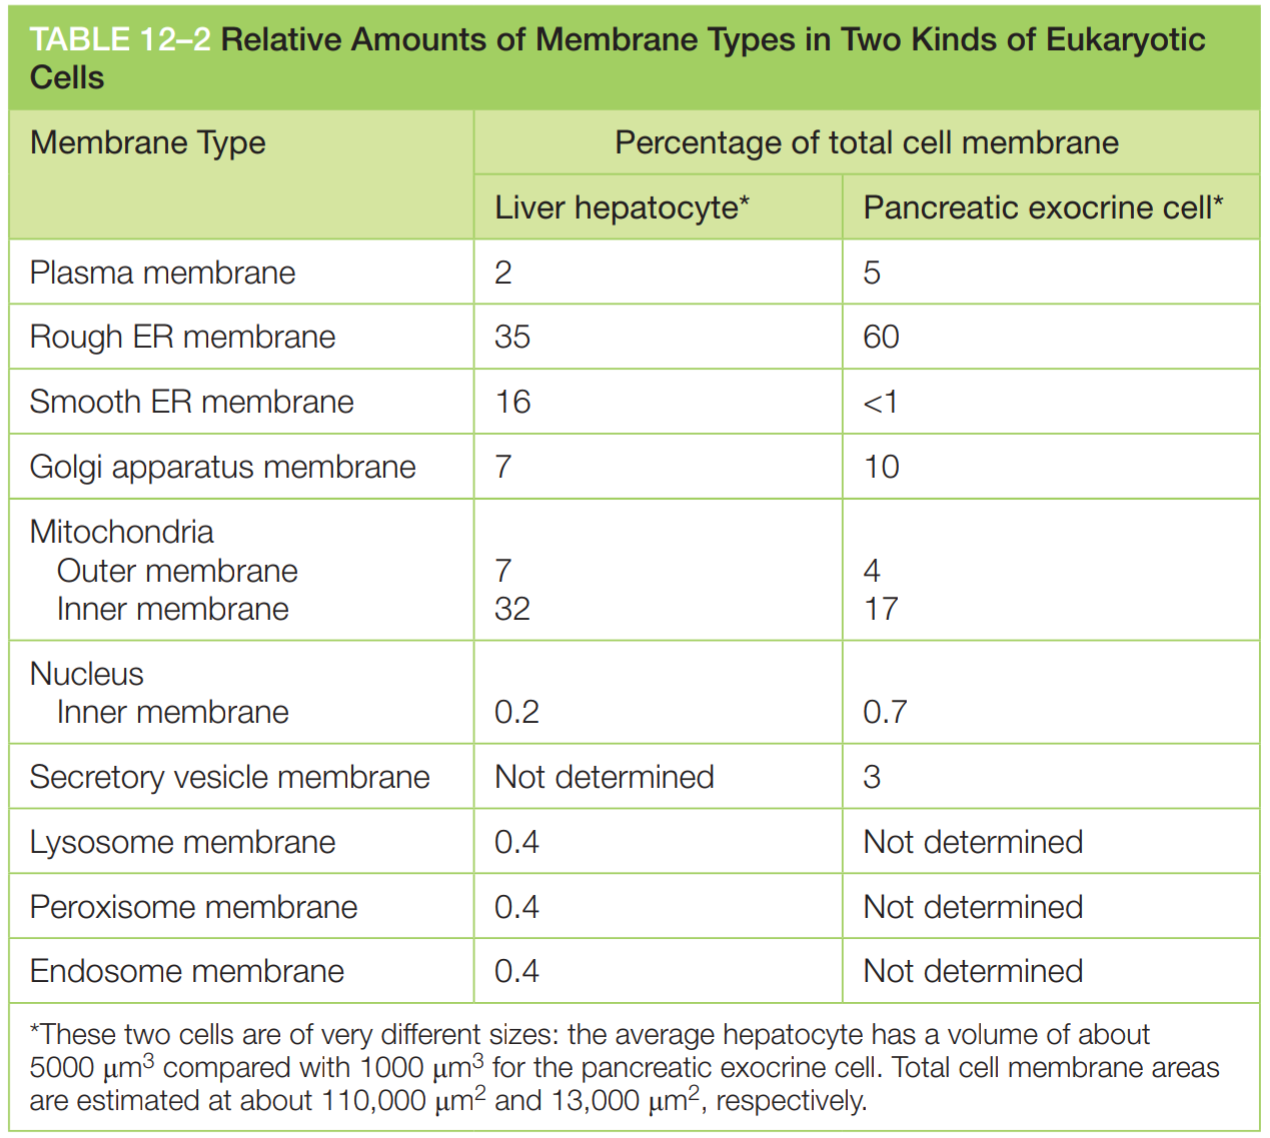
\includegraphics[scale=0.45]{images/table12-2.png}
        \end{center}
        \vspace{-1cm}
    \end{itemize}

    \hypertarget{12.1.2}{\subsection*{Topological Relationships of Organelles and Protein Movement}}
    \begin{itemize}
        \item Typical present-day eukaryotic cells are 10-30 times larger in linear dimension and 1000-10,000 times greater in volume than typical bacterium such as \textit{E. coli}.
        \item Evolutionary schemes suggest four distinct organelle families: 
            \begin{enumerate}
                \item The nucleus and cytosol.
                \item All organelles that function in the secretory and endocytic pathways. 
                \item Mitochondria
                \item Plastids (in plants)
            \end{enumerate}
        \item \textbf{Sorting signals}: particular amino acid sequences that direct delivery to locations outside the cytosol or to organelle surfaces.
        \item There are three fundamentally different ways by which proteins move:
        \begin{multicols}{2}
           
            \begin{enumerate}
                \item \textbf{Gated transport}: movement of proteins and RNA between the cytosol and the nucleus through nuclear pore complexes.
                \item \textbf{Protein translocation}: transmembrane proteins that directly transport specific proteins across a membrane from the cytosol into a topologically distinct space.
                \item \textbf{Vesicular transport}: membrane   enclosed transport intermediates ferry proteins from one topologically equivalent compartment to another. 
            \end{enumerate}
        \begin{center}
            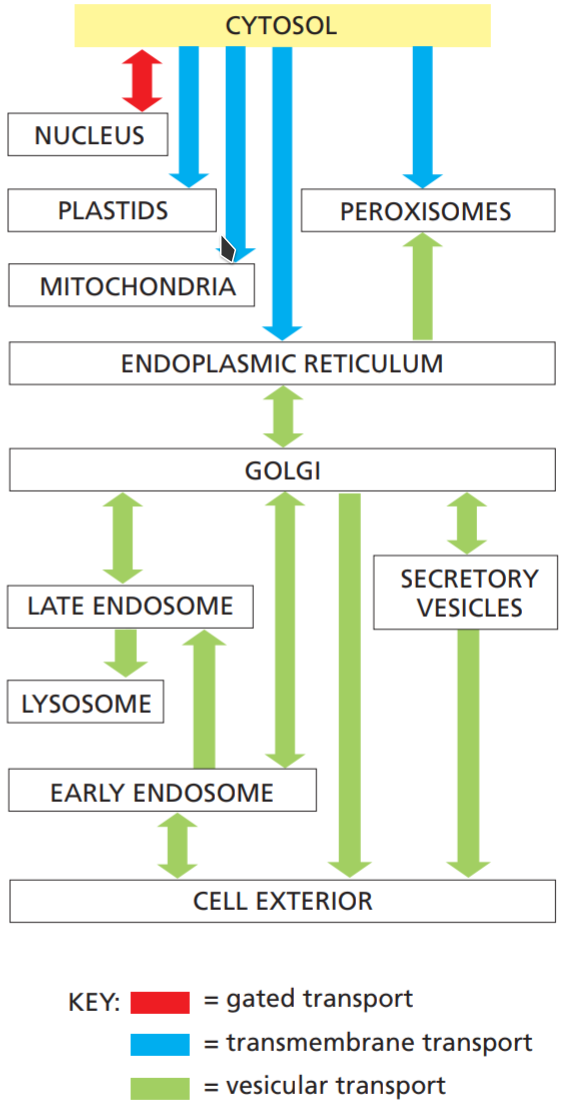
\includegraphics[scale=0.5]{images/fig12-5.png}
        \end{center}
        \end{multicols}
        \item \textit{Sorting receptors}: the site at which sorting signals are recognized for transport.
    \end{itemize}

    \hypertarget{12.1.3}{\subsection*{Signal Sequencs and Sorting Receptors}}
    \begin{itemize}
        \item Most protein sorting signals involved in transmembrane transport reside in amino acids sequences typically 15-60 residues long.
        \item Signal sequences are often found at the N-terminus of the polypeptide chain. 
        \item \textbf{Signal peptidases}: enzyme responsible for the removal the the signal sequence after the protein sorting process is complete.
        \item Sorting signals can be composed of multiple internal amino acid sequences that form a specific three-dimensional arrangement called \textbf{signal patches}, which are sometimes used for nuclear import and in vesicular transport.
        \item Proteins destined for the ER usually have a signal sequence at their N-terminus which are composed of about 5-10 hydrophobic amino acids and will remain in the ER if they have a specific sequence of four amino acids at their C-terminus.
        \item Most organelles cannot be constructed \textit{De novo}: they require information in the organelle itself, and enlarge and separate themselves during cell division. 
    \end{itemize}

    \hypertarget{12.1.r}{}

    \begin{probbox}{Compartmentalization of Cells: Summary}\end{probbox}
        Eukaryotic cells contain intracellular membrane-enclosed organelles that make up nearly half the cell’s total volume. The main ones present in all eukaryotic cells are the endoplasmic reticulum, Golgi apparatus, nucleus, mitochondria, lysosomes, endosomes, and peroxisomes; plant cells also contain plastids such as chloroplasts. These organelles contain distinct sets of proteins, which mediate each organelle’s unique function.\par 
        \vspace{10 pt}
        Each newly synthesized organelle protein must find its way from a ribosome in the cytosol, where the protein is made, to the organelle where it functions. It does so by following a specific pathway, guided by sorting signals in its amino acid sequence that function as either signal sequences or signal patches. Sorting signals are recognized by complementary sorting receptors, which deliver the protein to the appropriate target organelle. Proteins that function in the cytosol do not contain sorting signals and therefore remain there after they are synthesized.\par
        \vspace{10pt}
        During cell division, organelles such as the ER and mitochondria are distributed to each daughter cell. These organelles contain information that is required for their construction, and so they cannot be made de novo.
}\end{secbox}

\hypertarget{12.2}{}
\begin{secbox}{\hyperlink{12}{Transport of Between Nucleus and Cytosol}}{
    \hypertarget{12.2.1}{\subsection*{Basic Transport and the Nuclear Pore Complexes}}
    \begin{itemize}
        \item \textbf{Nuclear envelope}: encloses the DNA and defines the nuclear compartment and consists of two concentric membranes that are penetrated by nuclear pore complexes.
        \item \textbf{Inner nuclear membrane}: contains proteins that act as binding sites for chromosomes and for the \textit{nuclear lamina}, which is a protein meshwork that provides structural support for the nuclear envelope and an anchoring  site for chromosomes and the cytoplasmic cytoskeleton.
        \item \textbf{Outer nuclear membrane}: surrounds the inner membrane and is continuous with the membrane of the ER.
        \item \textit{Perinuclear space}: the space between the inner and outer nuclear membranes and is continuos with the ER lumen.
        \item \textbf{Nuclear pore complexes (NPCs)}: a large and elaborate protein complex that perforate the nuclear envelope and is composed of approximately 30 different proteins, or \textbf{Nucleoporins}.
        \item The nuclear envelope of a typical mammalian cell contains 3-4k NPCs, although it has a range from a few hundred in glial cells to over 20k in Purkinje neurons. 
        \item Each NPC can bidirectionally transport up to 1k macromolecules per second.
    \end{itemize}

    \hypertarget{12.2.2}{\subsection*{Nuclear Locolization Signals}}
    \begin{itemize}
        \item \textbf{Nuclear localization signals (NLSs)}: responsible for the selectivity of the active nuclear import process.
        \item An entire complex will be imported into the nucleus as long as one of the protein subunits of a multicomponent complex displays a nuclear localization signal.
    \end{itemize}

    \hypertarget{12.2.3}{\subsection*{Nuclear Import Receptors}}
    \begin{itemize}
        \item \textbf{Nuclear Import Receptors}: also known as importins, must recognize nuclear localization signals in order to initiate nuclear import. 
        \item Importins do not always bind to nuclear proteins directly.
        \item There are variety of ways cells can use imports receptors and adaptors that allow them to recognize the broad repertoire of nuclear localization signals. 
    \end{itemize} 

    \hypertarget{12.2.4}{\subsection*{Nuclear Export}}
    \begin{itemize}
        \item Nuclear export works like nuclear import, but in reverse.
        \item The transport system relies of \textbf{nuclear export signals} on the macromolecules to be exported, as well as complementary \textbf{nuclear export receptors}, or \textit{exportins}. 
    \end{itemize}
    
    \hypertarget{12.2.5}{\subsection*{Ran GTPase}}
    \begin{itemize}
        \item \textbf{Ran}: a GTP-bound form a monomeric GTPase that fuels nuclear import and export by harnessing energy stored in the concentration gradient.
        \item Ran is a molecular switch that can exist in two conformational states, depending on whether GDP or GTp is bound.
        \item The gradient of the two conformation forms of Ran drives nuclear transport in the appropriate direction.\par 
        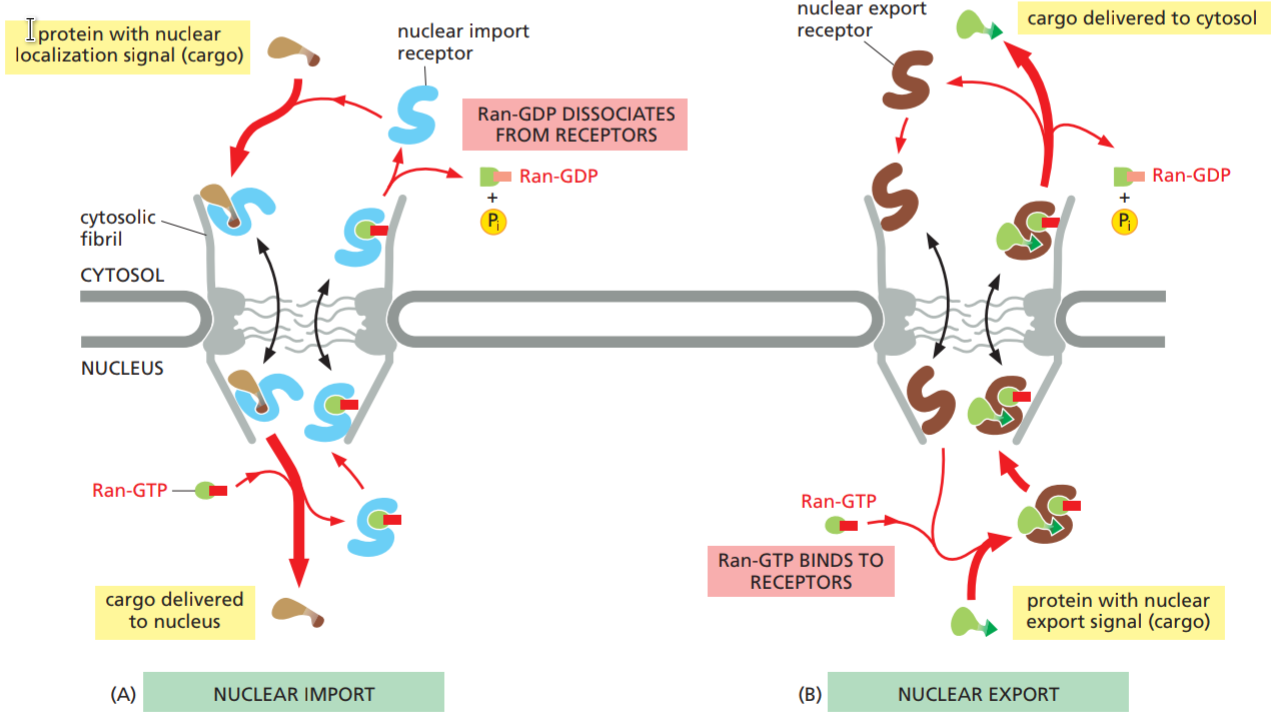
\includegraphics[width=\linewidth]{images/fig12-13.png}
        \item Some proteins contain both nuclear localization signals and nuclear export signals and will continually shuttle back and forth between the nucleus and cytosol.
    \end{itemize}
    
    
    \hypertarget{12.2.6}{\subsection*{Nuclear Envelope During Mitosis}}
    \begin{itemize}
        \item \textbf{Nuclear Lamina}: a meshwork of interconnected protein subunits called \textbf{nuclear lamins} located oon the nuclear side of the inner nuclear membrane.
        \item The nuclear lamina gives shape and stability to the nuclear envelope, to which it is anchored by attachment to both the NPCs and transmembrane proteins of hte inner nuclear membrane.
        \item Phosphorylation of lamins and NPC proteins break disassemble the nuclear envelope during mitosis.
        \item The chromosomes of the mitotic cells are released and surrounded by a cloud of Ran-GTP. 
        \item The previously freed NPCs now surround the new chromosome while the inner nuclear membrane proteins and dephosphorylated lamins bind to the chromatin.
        \item ER membranes then wrap around groups of chromosomes until they form a sealed nuclear envelope and the NPCs start actively re-importing proteins that contain nuclear localization signals.
        \item Eventually, as decondensation progresses, these  structures fuse to form a single complete nucleus.\par
        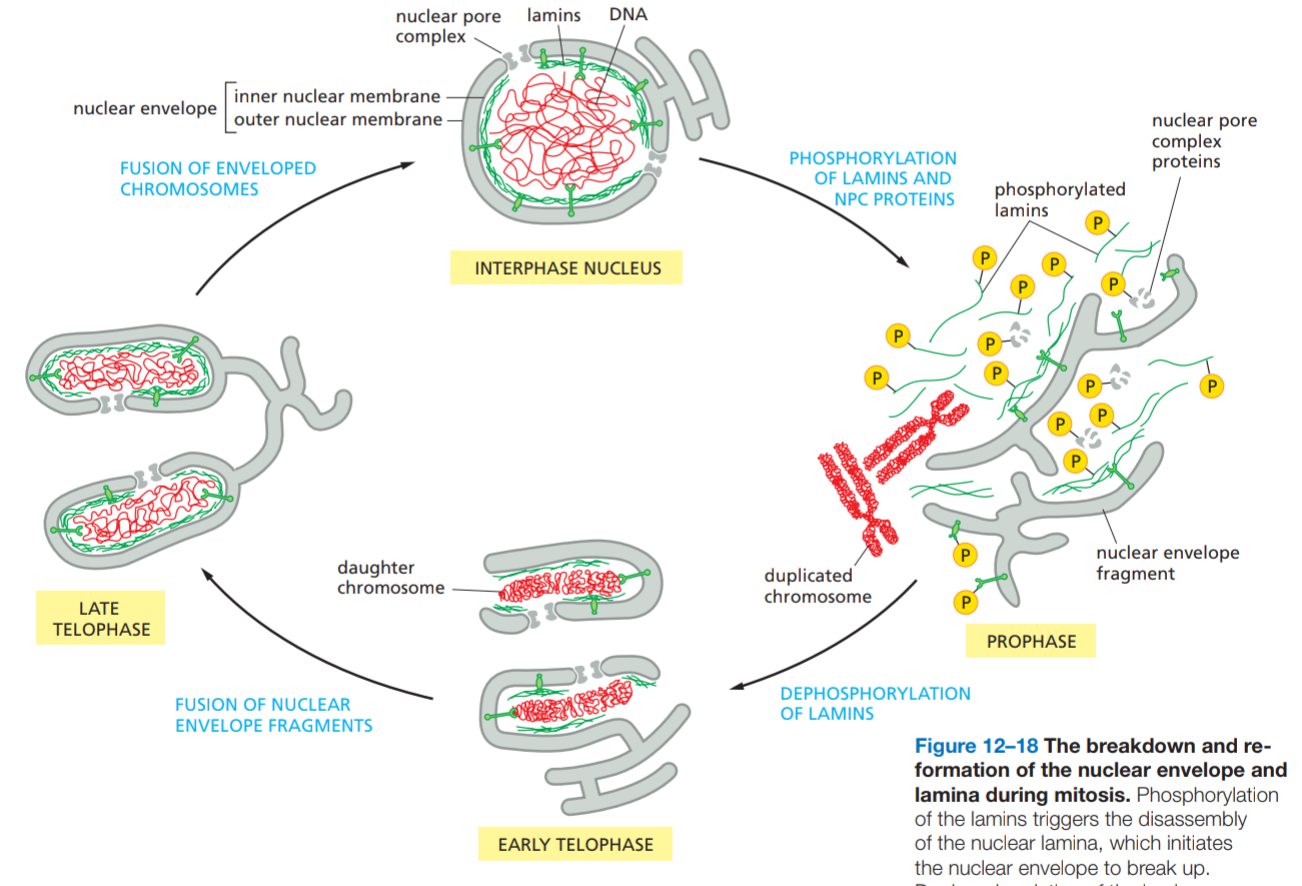
\includegraphics[width=\linewidth]{images/fig12-18.png}
    \end{itemize}
    
    \hypertarget{12.2.r}{}
    \begin{probbox}{Transport of Between Nucleus and Cytosol: Summary}\end{probbox}

    The nuclear envelope consists of an inner and an outer nuclear membrane that are continuous with each other and with the ER membrane, and the space between the inner and outer nuclear membrane is continuous with the ER lumen. RNA molecules, which are made in the nucleus, and ribosomal subunits, which are assembled there, are exported to the cytosol; in contrast, all the proteins that function in the nucleus are synthesized in the cytosol and are then imported. The extensive traffic of materials between the nucleus and cytosol occurs through nuclear pore complexes (NPCs), which provide a direct passageway across the nuclear envelope. Small molecules diffuse passively through the NPCs, but large macromolecules have to be actively transported. \par 
    \vspace{12pt}
    Proteins containing nuclear localization signals are actively transported into the nucleus through NPCs, while proteins containing nuclear export signals are transported out of the nucleus to the cytosol. Some proteins, including the nuclear import and export receptors, continually shuttle between the cytosol and nucleus. The monomeric GTPase Ran provides both the free energy and the directionality for nuclear transport. Cells regulate the transport of nuclear proteins and RNA molecules through the NPCs by controlling the access of these molecules to the transport machinery. Newly transcribed messenger RNA and ribosomal RNA are exported from the nucleus as parts of large ribonucleoprotein complexes. Because nuclear localization signals are not removed, nuclear proteins can be imported repeatedly, as is required each time that the nucleus reassembles after mitosis.
}\end{secbox}

\hypertarget{12.3}{}
\begin{secbox}{\hyperlink{12}{Transport of Proteins into Mitochondria and Chloroplasts}}{
    \hypertarget{12.3.1}{\subsection*{Translocation into Mitochondria}}
    \begin{itemize}
        \item Proteins imported into mitochondria are usually taken up from the cytosol within seconds or minutes of their release from ribosomes.
        \item Mitochondrial proteins are first fully synthesizes as \textbf{mitochondial precursor proteins} in the cytosol and then translocated into the mitochondria by a \textit{post-translational} mechanism.
        \item \textbf{Protein translocators}: multisubunit protein complexes that mediate protein movement across mitochondial membranes.
        \item \textbf{TOM complex}: transfers proteins across the outer membrane.
        \item \textbf{TIM complexes}: two complexes that transfer proteins across the inner membrane.
        \item \textbf{SAM complex}: helps proteins to fold properly in the outer membranes.
        \item \textit{TIM23}: transports some soluble proteins into the matrix space and helps to insert transmembrane proteins into the inner membrane.
        \item \textit{TIM22}: mediates the insertion of a subclass of inner membrane proteins, including the transporter that moves ADP,ATP, and phosphate in and out of mitochondria.
        \item \textbf{OXA complex}: mediates the insertion inner membrane proteins that are synthesized within mitochondria, as well as some imported inner membrane proteins.\par 
        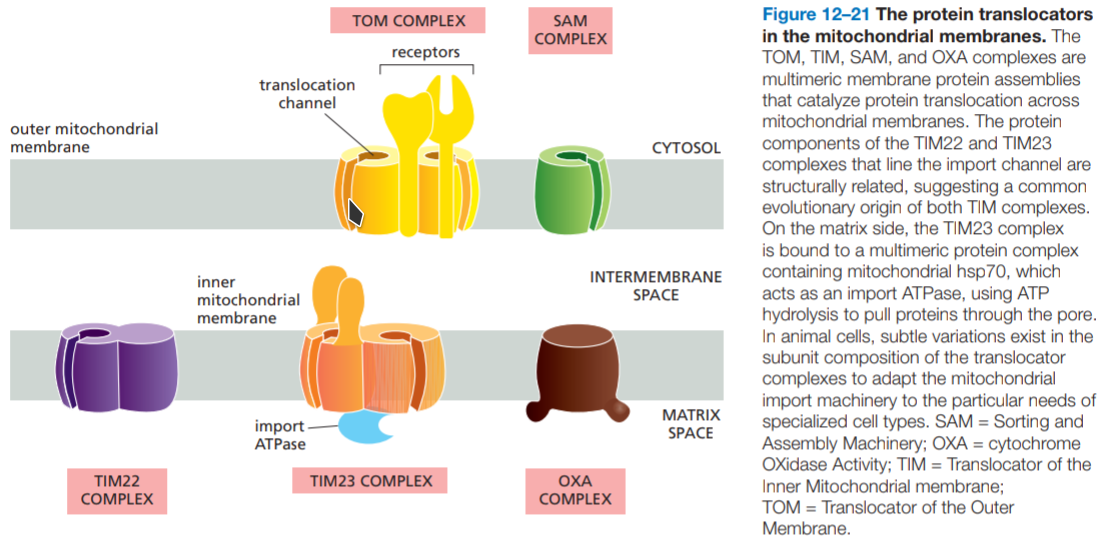
\includegraphics[width=\linewidth]{images/fig12-21.png}
    \end{itemize}
        

    \hypertarget{12.3.2}{\subsection*{Mitochondrial Precursor Proteins}}
    \begin{itemize}
        \item Mitochondrial precursor proteins do not fold into their native structures after they are synthesized; instead, they remain unfolded in the cytosol through interactions with other proteins.
    \end{itemize}

    \hypertarget{12.3.3}{\subsection*{Protein Import into the Matrix Space}}
    \begin{itemize}
        \item The first requirement for energy occurs at the initial stage of translocation process, when the unfolded precursor protein interacts with the import receptors of the TOM complex.
        \item Further translocation through the TIM complex requires there to be membrane potential, which is made from pumping \ch{H^+} from the matrix space to the intermembrane space via electron transport processes.
        \item \textbf{Mitochondrial hsp70}: part of a multisubunit protein assembly that is bound to the matrix side of TIM23 complex and acts as a motor to pull the precursor protein into the matrix space.
        \item \textit{hsp60}: helps the unfolded polypeptide chian to fold by binding and releasing it through cycles of ATP hydrolysis.
    \end{itemize}

    \hypertarget{12.3.4}{\subsection*{Bacterial and Mitochondrial Insertion of Poroins into Outer Membrane}}
    \begin{itemize}
        \item \textbf{Porins}: pore-forming \(\beta\)-barrel proteins on the outer mitochondrial membrane.
        \item Unlike other outer membrane proteins, porins are instead first transported unfolded into the intermembrane space where they bind to specialized chaperone proteins that keep the porins from aggregating. They then bind to SAM complex which inserts them into the outer membrane.
        \item This conserved pathway for inserting \(\beta\)-barrel proteins further underscores the endosymbiotic origin of mitochondria.
    \end{itemize}
    
    \hypertarget{12.3.r}{}
    \begin{probbox}{Transport of Proteins into Mitochondria and Chloroplasts: Summary}\end{probbox}
    Although mitochondria and chloroplasts have their own genetic systems, they produce only a small proportion of their own proteins. Instead, the two organelles import most of their proteins from the cytosol, using similar mechanisms. In both cases, proteins are transported in an unfolded state across both outer and inner membranes simultaneously into the matrix space or stroma. Both ATP hydrolysis and a membrane potential across the inner membrane drive translocation into mitochondria, whereas GTP and ATP hydrolysis drive translocation into chloroplasts. Chaperone proteins of the cytosolic hsp70 family maintain the precursor proteins in an unfolded state, and a second set of hsp70 proteins in the matrix space or stroma pulls the polypeptide chain into the organelle. Only proteins that contain a specific signal sequence are translocated. The signal sequence can either be located at the N-terminus and cleaved off after import or be internal and retained. Transport into the inner membrane sometimes uses a second, hydrophobic signal sequence that is unmasked when the first signal sequence is removed. In chloroplasts, import from the stroma into the thylakoid can occur by several routes, distinguished by the chaperones and energy source used.
}\end{secbox}

\hypertarget{12.4}{}
\begin{secbox}{\hyperlink{12}{Peroxisomes}}{
    \hypertarget{12.4.1}{\subsection*{Peroxisomes Use of Molecular Oxygen and Hydrogen Peroxide}}
    \begin{itemize}
        \item Peroxisomes are only surrounded by a single membrane, do not contain DNA or ribosomes, and acquire most proteins by selective import from the cytosol.
        \item Virtually all eukaryotic cells have peroxisomes.
        \item Peroxisomes contain oxidative enzymes such as catalase and urate oxidase at very high concentrations.
        \item A major function of the oxidation reactions performed in peroxisomes is the breakdown of fatty acids molecules.
        \item An essential biosynthetic function of animal peroxisomes is to catalyze the first reaction in the formation of \textit{plasmalogens}, which are the most abundant class of phospholipids in myelin.
    \end{itemize}

    \hypertarget{12.4.2}{\subsection*{Import of Proteins into Peroxisomes}}
    \begin{itemize}
        \item A specific sequence of three amino acids (Ser-Lys-Leu) located at the C-terminus functions as an import signal for many peroxisomal proteins.
        \item \textbf{Peroxins}: distinct proteins that participate in the import process, which is driven by ATP hydrolysis.
    \end{itemize}

    \hypertarget{12.4.r}{}
    \begin{probbox}{Peroxisomes: Summary}\end{probbox}
    Peroxisomes are specialized for carrying out oxidation reactions using molecular oxygen. They generate hydrogen peroxide, which they employ for oxidative purposes—and contain catalase to destroy the excess. Like mitochondria and plastids, peroxisomes are self-replicating organelles. Because they do not contain DNA or ribosomes, however, all of their proteins are encoded in the cell nucleus. Some of these proteins are conveyed to peroxisomes via peroxisomal precursor vesicles that bud from the ER, but most are synthesized in the cytosol and directly imported. A specific sequence of three amino acids near the C-terminus of many of the latter proteins functions as a peroxisomal import signal. The mechanism of protein import differs from that of mitochondria and chloroplasts, in that even oligomeric proteins are imported from the cytosol without unfolding.
}\end{secbox}

\hypertarget{12.5}{}
\begin{secbox}{\hyperlink{12}{The Endoplasmic Reticulum}}{
    \hypertarget{12.5.1}{\subsection*{ER Strucutre and Function}}
    \begin{itemize}
        \item
    \end{itemize}

    \hypertarget{12.5.2}{\subsection*{ER Signal Sequences}}
    \begin{itemize}
        \item
    \end{itemize}

    \hypertarget{12.5.3}{\subsection*{Signal-Recognition Particle}}
    \begin{itemize}
        \item
    \end{itemize}

    \hypertarget{12.5.4}{\subsection*{Polypeptide Chain Transport and the Translocator}}
    \begin{itemize}
        \item
    \end{itemize}
    
    \hypertarget{12.5.5}{\subsection*{Translocation Across the ER and More on Signal Seuqences}}
    \begin{itemize}
        \item
    \end{itemize}
    
    \hypertarget{12.5.6}{\subsection*{ER Tail-Anchored Proteins Integration}}
    \begin{itemize}
        \item
    \end{itemize}
    
    \hypertarget{12.5.7}{\subsection*{Folding and Assembling of Translocated Polypeptide Chains}}
    \begin{itemize}
        \item
    \end{itemize}
    
    \hypertarget{12.5.8}{\subsection*{Protein Synthesis in the Rough ER}}
    \begin{itemize}
        \item
    \end{itemize}
    
    \hypertarget{12.5.9}{\subsection*{Oligosaccharide Tags and Protein Folding}}
    \begin{itemize}
        \item
    \end{itemize}
    
    \hypertarget{12.5.10}{\subsection*{The ER Assembles Most Lipid Bilayers}}
    \begin{itemize}
        \item
    \end{itemize}
    
    \hypertarget{12.5.r}{} 
    \begin{probbox}{The Endoplasmic Reticulum: Summary}\end{probbox}
    The extensive ER network serves as a factory for the production of almost all of the cell’s lipids. In addition, a major portion of the cell’s protein synthesis occurs on the cytosolic surface of the rough ER: virtually all proteins destined for secretion or for the ER itself, the Golgi apparatus, the lysosomes, the endosomes, and the plasma membrane are first imported into the ER from the cytosol. In the ER lumen, the proteins fold and oligomerize, disulfide bonds are formed, and N-linked oligosaccharides are added. The pattern of N-linked glycosylation is used to indicate the extent of protein folding, so that proteins leave the ER only when they are properly folded. Proteins that do not fold or oligomerize correctly are translocated back into the cytosol, where they are deglycosylated, polyubiquitylated, and degraded in proteasomes. If misfolded proteins accumulate in excess in the ER, they trigger an unfolded protein response, which activates appropriate genes in the nucleus to help the ER cope. \par 
    \vspace{10pt}
    Only proteins that carry a special ER signal sequence are imported into the ER. The signal sequence is recognized by a signal-recognition particle (SRP), which binds both the growing polypeptide chain and the ribosome and directs them to a receptor protein on the cytosolic surface of the rough ER membrane. This binding to the ER membrane initiates the translocation process that threads a loop of polypeptide chain across the ER membrane through the hydrophilic pore of a protein translocator. \par 
    \vspace{10pt}
    Soluble proteins—destined for the ER lumen, for secretion, or for transfer to the lumen of other organelles—pass completely into the ER lumen. Transmembrane proteins destined for the ER or for other cell membranes are translocated part way across the ER membrane and remain anchored there by one or more membrane-spanning \(\alpha\)-helical segments in their polypeptide chains. These hydrophobic portions of the protein can act either as start-transfer or stop-transfer signals during the translocation process. When a polypeptide contains multiple, alternating start-transfer and stop-transfer signals, it will pass back and forth across the bilayer multiple times as a multipass transmembrane protein. \par
    \vspace{10pt}
    The asymmetry of protein insertion and glycosylation in the ER establishes the sidedness of the membranes of all the other organelles that the ER supplies with membrane proteins.
}\end{secbox}

%\endgroup
%  ^^^^^^^^^^^^^^^^^^^^^^^^^^^^^^^^^    Chapter 12    ^^^^^^^^^^^^^^^^^^^^^^^^^^^^^^^^^  %  
%%%%%%%%%%%%%%%%%%%%%%%%%%%%%%%%%%%%%%%%%%%%%%%%%%%%%%%%%%%%%%%%%%%%%%%%%%%%%%%%%%%%%%%%%%

%%%%%%%%%%%%%%%%%%%%%%%%%%%%%%%%%%%%%%%%%%%%%%%%%%%%%%%%%%%%%%%%%%%%%%%%%%%%%%%%%%%%%%%%%%
%  vvvvvvvvvvvvvvvvvvvvvvvvvvvvvvvvv    Chapter 13    vvvvvvvvvvvvvvvvvvvvvvvvvvvvvvvvv  %
%\begingroup

%\endgroup
%  ^^^^^^^^^^^^^^^^^^^^^^^^^^^^^^^^^    Chapter 13    ^^^^^^^^^^^^^^^^^^^^^^^^^^^^^^^^^  %  
%%%%%%%%%%%%%%%%%%%%%%%%%%%%%%%%%%%%%%%%%%%%%%%%%%%%%%%%%%%%%%%%%%%%%%%%%%%%%%%%%%%%%%%%%%

%%%%%%%%%%%%%%%%%%%%%%%%%%%%%%%%%%%%%%%%%%%%%%%%%%%%%%%%%%%%%%%%%%%%%%%%%%%%%%%%%%%%%%%%%%
%  vvvvvvvvvvvvvvvvvvvvvvvvvvvvvvvvv    Chapter 14    vvvvvvvvvvvvvvvvvvvvvvvvvvvvvvvvv  %
%\begingroup

%\endgroup
%  ^^^^^^^^^^^^^^^^^^^^^^^^^^^^^^^^^    Chapter 14    ^^^^^^^^^^^^^^^^^^^^^^^^^^^^^^^^^  %  
%%%%%%%%%%%%%%%%%%%%%%%%%%%%%%%%%%%%%%%%%%%%%%%%%%%%%%%%%%%%%%%%%%%%%%%%%%%%%%%%%%%%%%%%%%

%%%%%%%%%%%%%%%%%%%%%%%%%%%%%%%%%%%%%%%%%%%%%%%%%%%%%%%%%%%%%%%%%%%%%%%%%%%%%%%%%%%%%%%%%%
%  vvvvvvvvvvvvvvvvvvvvvvvvvvvvvvvvv    Chapter 15    vvvvvvvvvvvvvvvvvvvvvvvvvvvvvvvvv  %
%\begingroup

%\endgroup
%  ^^^^^^^^^^^^^^^^^^^^^^^^^^^^^^^^^    Chapter 15    ^^^^^^^^^^^^^^^^^^^^^^^^^^^^^^^^^  %  
%%%%%%%%%%%%%%%%%%%%%%%%%%%%%%%%%%%%%%%%%%%%%%%%%%%%%%%%%%%%%%%%%%%%%%%%%%%%%%%%%%%%%%%%%%

%%%%%%%%%%%%%%%%%%%%%%%%%%%%%%%%%%%%%%%%%%%%%%%%%%%%%%%%%%%%%%%%%%%%%%%%%%%%%%%%%%%%%%%%%%
%  vvvvvvvvvvvvvvvvvvvvvvvvvvvvvvvvv    Chapter 16    vvvvvvvvvvvvvvvvvvvvvvvvvvvvvvvvv  %
%\begingroup

%\endgroup
%  ^^^^^^^^^^^^^^^^^^^^^^^^^^^^^^^^^    Chapter 16    ^^^^^^^^^^^^^^^^^^^^^^^^^^^^^^^^^  %  
%%%%%%%%%%%%%%%%%%%%%%%%%%%%%%%%%%%%%%%%%%%%%%%%%%%%%%%%%%%%%%%%%%%%%%%%%%%%%%%%%%%%%%%%%%

%%%%%%%%%%%%%%%%%%%%%%%%%%%%%%%%%%%%%%%%%%%%%%%%%%%%%%%%%%%%%%%%%%%%%%%%%%%%%%%%%%%%%%%%%%
%  vvvvvvvvvvvvvvvvvvvvvvvvvvvvvvvvv    Chapter 17    vvvvvvvvvvvvvvvvvvvvvvvvvvvvvvvvv  %
%\begingroup

%\endgroup
%  ^^^^^^^^^^^^^^^^^^^^^^^^^^^^^^^^^    Chapter 17    ^^^^^^^^^^^^^^^^^^^^^^^^^^^^^^^^^  %  
%%%%%%%%%%%%%%%%%%%%%%%%%%%%%%%%%%%%%%%%%%%%%%%%%%%%%%%%%%%%%%%%%%%%%%%%%%%%%%%%%%%%%%%%%%

%%%%%%%%%%%%%%%%%%%%%%%%%%%%%%%%%%%%%%%%%%%%%%%%%%%%%%%%%%%%%%%%%%%%%%%%%%%%%%%%%%%%%%%%%%
%  vvvvvvvvvvvvvvvvvvvvvvvvvvvvvvvvv    Chapter 19    vvvvvvvvvvvvvvvvvvvvvvvvvvvvvvvvv  %
%\begingroup

%\endgroup
%  ^^^^^^^^^^^^^^^^^^^^^^^^^^^^^^^^^    Chapter 19    ^^^^^^^^^^^^^^^^^^^^^^^^^^^^^^^^^  %  
%%%%%%%%%%%%%%%%%%%%%%%%%%%%%%%%%%%%%%%%%%%%%%%%%%%%%%%%%%%%%%%%%%%%%%%%%%%%%%%%%%%%%%%%%%

%%%%%%%%%%%%%%%%%%%%%%%%%%%%%%%%%%%%%%%%%%%%%%%%%%%%%%%%%%%%%%%%%%%%%%%%%%%%%%%%%%%%%%%%%%
%  vvvvvvvvvvvvvvvvvvvvvvvvvvvvvvvvv    Chapter 20    vvvvvvvvvvvvvvvvvvvvvvvvvvvvvvvvv  %
%\begingroup

%\endgroup
%  ^^^^^^^^^^^^^^^^^^^^^^^^^^^^^^^^^    Chapter 20    ^^^^^^^^^^^^^^^^^^^^^^^^^^^^^^^^^  %  
%%%%%%%%%%%%%%%%%%%%%%%%%%%%%%%%%%%%%%%%%%%%%%%%%%%%%%%%%%%%%%%%%%%%%%%%%%%%%%%%%%%%%%%%%%

%%%%%%%%%%%%%%%%%%%%%%%%%%%%%%%%%%%%%%%%%%%%%%%%%%%%%%%%%%%%%%%%%%%%%%%%%%%%%%%%%%%%%%%%%%
%  vvvvvvvvvvvvvvvvvvvvvvvvvvvvvvvvv    Chapter 22    vvvvvvvvvvvvvvvvvvvvvvvvvvvvvvvvv  %
%\begingroup

%\endgroup
%  ^^^^^^^^^^^^^^^^^^^^^^^^^^^^^^^^^    Chapter 22    ^^^^^^^^^^^^^^^^^^^^^^^^^^^^^^^^^  %  
%%%%%%%%%%%%%%%%%%%%%%%%%%%%%%%%%%%%%%%%%%%%%%%%%%%%%%%%%%%%%%%%%%%%%%%%%%%%%%%%%%%%%%%%%%

%%%%%%%%%%%%%%%%%%%%%%%%%%%%%%%%%%%%%%%%%%%%%%%%%%%%%%%%%%%%%%%%%%%%%%%%%%%%%%%%%%%%%%%%%%
%  vvvvvvvvvvvvvvvvvvvvvvvvvvvvvvvvv    Chapter 24    vvvvvvvvvvvvvvvvvvvvvvvvvvvvvvvvv  %
%\begingroup

%\endgroup
%  ^^^^^^^^^^^^^^^^^^^^^^^^^^^^^^^^^    Chapter 24    ^^^^^^^^^^^^^^^^^^^^^^^^^^^^^^^^^  %  
%%%%%%%%%%%%%%%%%%%%%%%%%%%%%%%%%%%%%%%%%%%%%%%%%%%%%%%%%%%%%%%%%%%%%%%%%%%%%%%%%%%%%%%%%%
\end{document}